\documentclass[11pt]{article}

\usepackage[utf8]{inputenc}
\usepackage[T1]{fontenc}
\usepackage{amsmath,amssymb,amsfonts}
\usepackage{bm}
\usepackage{geometry}
\usepackage{graphicx}
\usepackage{hyperref}
\usepackage{tikz}

\graphicspath{{../figures/}}

\usetikzlibrary{arrows.meta,calc,positioning}

\geometry{margin=1in}

\title{Boundary layer meshes in Gmsh}
\author{}
\date{}

\newcommand{\R}{\mathbb{R}}
\newcommand{\dd}{\mathrm{d}}
\newcommand{\bx}{\bm{x}}
\newcommand{\bu}{\bm{u}}
\newcommand{\bxi}{\bm{\xi}}
\newcommand{\bX}{\bm{X}}
\newcommand{\bG}{\bm{G}}
\newcommand{\bJ}{\bm{J}}

\begin{document}
\maketitle

\begin{abstract}
We present a boundary-layer meshing procedure for Gmsh. The method starts from
an existing watertight mesh and creates a layer of zero-thickness elements with
the correct topology on the selected curves, surfaces and volumes. These flat
elements are then pushed into the surrounding mesh with a robust smoothing and
untangling procedure, preserving the connectivity of the original mesh while
creating the required anisotropic boundary-layer cells. The construction is
designed to work in both two and three dimensions, and to provide a consistent
foundation for subsequent high-order boundary-layer meshes.
\end{abstract}

\section{Creation of the Flat Boundary-Layer Topology}

\subsection{Plugin Input}

The boundary-layer algorithm is implemented as a Gmsh plugin. It is deliberately
applied after the usual Gmsh mesh generation stage: the user first creates a
standard watertight mesh with the normal Gmsh workflow, and the plugin then
modifies this existing mesh. This is important in practice. The boundary-layer
procedure does not replace the CAD import, the curve and surface meshing, or the
volume meshing algorithms of Gmsh; it acts as a post-processing step on a valid
mesh and preserves the surrounding mesh connectivity as much as possible.

In two dimensions, the input is a list of faces where the mesh may be modified
and a list of curves from which the layer should be grown. In three dimensions,
the input is a list of volumes into which the layer should be inserted and a
list of boundary faces supporting the layer. The geometric parameters are the
total thickness, the size of the first layer, the growth ratio and the number of
smoothing layers. Optional parameters control the number of exact split layers
and the order of the final mesh.

The following example is representative of the two-dimensional case
\texttt{benchmarks/bl/3cw.geo}. The geometry and the initial mesh are generated
first. The boundary-layer plugin is then run on surface 16, starting from curves
1 to 7.

\begin{verbatim}
Mesh 2;
Mesh.MeshSizeFactor = 0.5;
Mesh.NumSubEdges = 10;

Plugin(BoundaryLayer).Surfaces = "16";
Plugin(BoundaryLayer).Curves = "1,2,3,4,5,6,7";

Plugin(BoundaryLayer).Thickness = 40;
Plugin(BoundaryLayer).Size = .3;
Plugin(BoundaryLayer).Ratio = 1.5;
Plugin(BoundaryLayer).SmoothingLayers = 5;
Plugin(BoundaryLayer).HighOrder = 2;

Plugin(BoundaryLayer).Run;
\end{verbatim}

In a three-dimensional case the analogous input is
\begin{verbatim}
Mesh 3;

Plugin(BoundaryLayer).Volumes = "1";
Plugin(BoundaryLayer).Surfaces = "7,8,9,10";

Plugin(BoundaryLayer).Thickness = 1./3.;
Plugin(BoundaryLayer).Size = 1./250.;
Plugin(BoundaryLayer).Ratio = 1.3;
Plugin(BoundaryLayer).SmoothingLayers = 4;
Plugin(BoundaryLayer).HighOrder = 2;

Plugin(BoundaryLayer).Run;
\end{verbatim}

These snippets are intentionally written in the \texttt{.geo} language, since
this is the most direct interface for users. The same options can also be set
through the Python API with \texttt{gmsh.plugin.setString} and
\texttt{gmsh.plugin.setNumber}.

\subsection{Example: the 3CW Airfoil}

As a first example we consider the \texttt{3cw} two-dimensional benchmark
distributed with Gmsh in \texttt{benchmarks/bl/3cw.geo}. The geometry contains a
single meshed surface, numbered 16, bounded by several spline curves. The
standard Gmsh mesh generation produces a watertight triangular surface mesh
without any boundary layer:
\[
  1795 \ \text{nodes}, \qquad 2491 \ \text{mesh elements}.
\]
On the test machine used here, the two-dimensional meshing time was
approximately \(1.1\times10^{-2}\) seconds.

\begin{figure}[htbp]
\centering
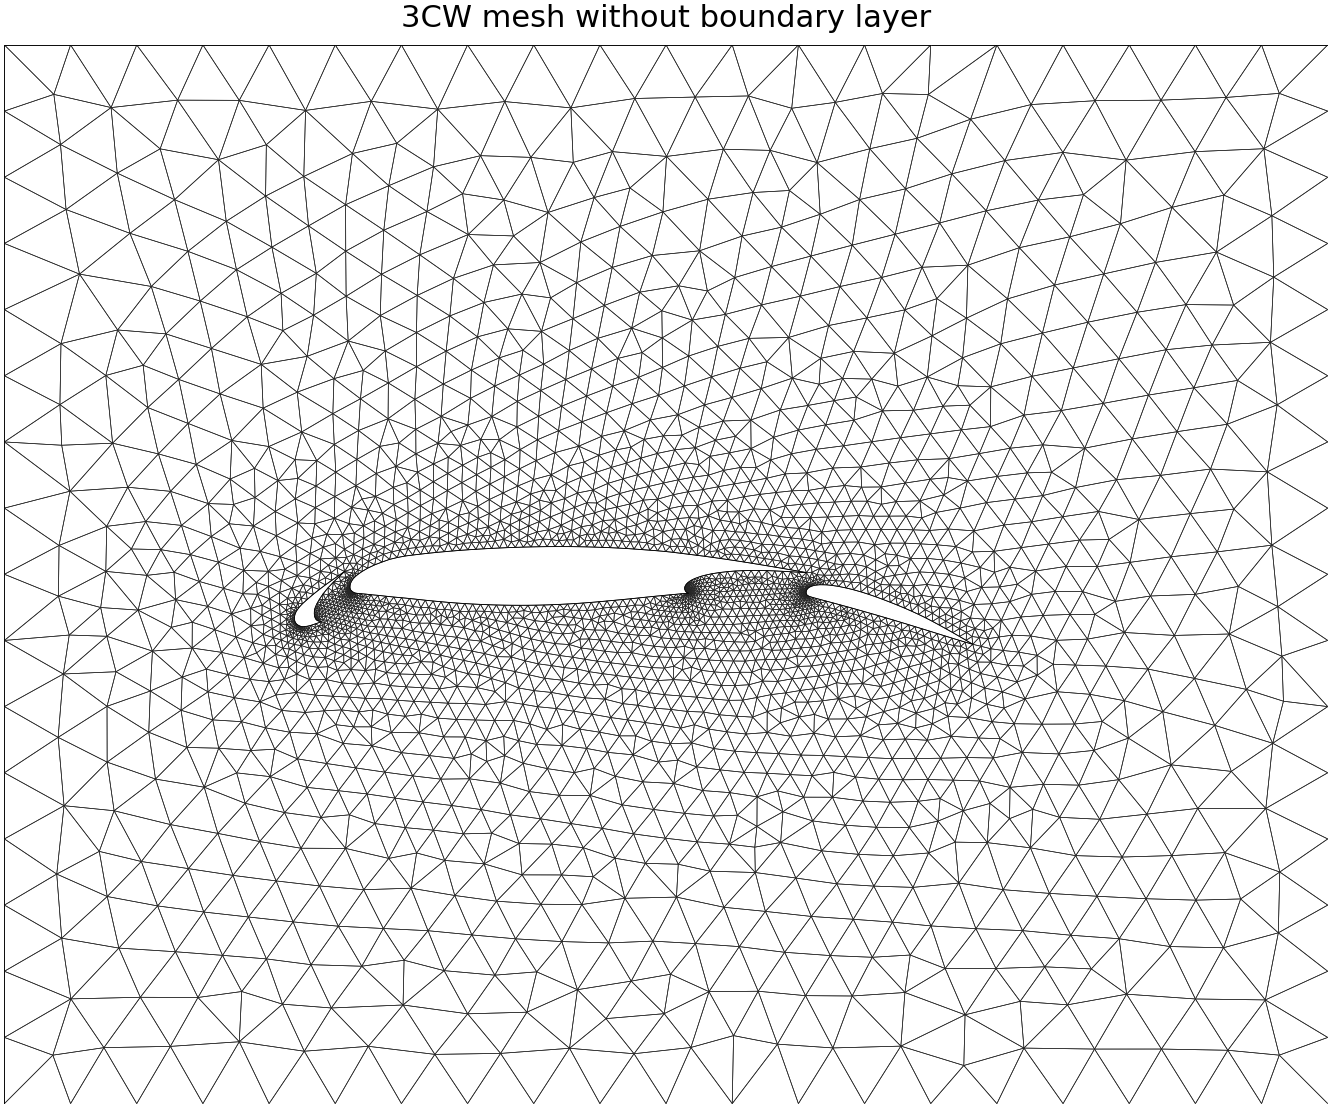
\includegraphics[width=0.82\linewidth]{../figures/3cw_no_bl.png}
\caption{Initial 3CW mesh generated by the standard Gmsh surface mesher.}
\label{fig:3cw-no-bl}
\end{figure}

The boundary layer is requested on the same surface, using curves 1 to 7 as the
support curves:
\begin{verbatim}
Mesh 2;

Plugin(BoundaryLayer).Surfaces = "16";
Plugin(BoundaryLayer).Curves = "1,2,3,4,5,6,7";

Plugin(BoundaryLayer).Thickness = 40;
Plugin(BoundaryLayer).Size = .3;
Plugin(BoundaryLayer).Ratio = 1.5;
Plugin(BoundaryLayer).SmoothingLayers = 5;
Plugin(BoundaryLayer).HighOrder = 2;

Plugin(BoundaryLayer).Run;
\end{verbatim}

Before showing the final graded layer, it is useful to isolate the elementary
operation performed by the plugin. If we set
\[
  \texttt{Size}=\texttt{Thickness}=40,
\]
the plugin creates and expands a single boundary-layer row. This is the
simplest way to visualize the first step: the wall edges are duplicated, the
zero-thickness quadrangles are created, and this single row is pushed into the
existing surface mesh.

\begin{figure}[htbp]
\centering
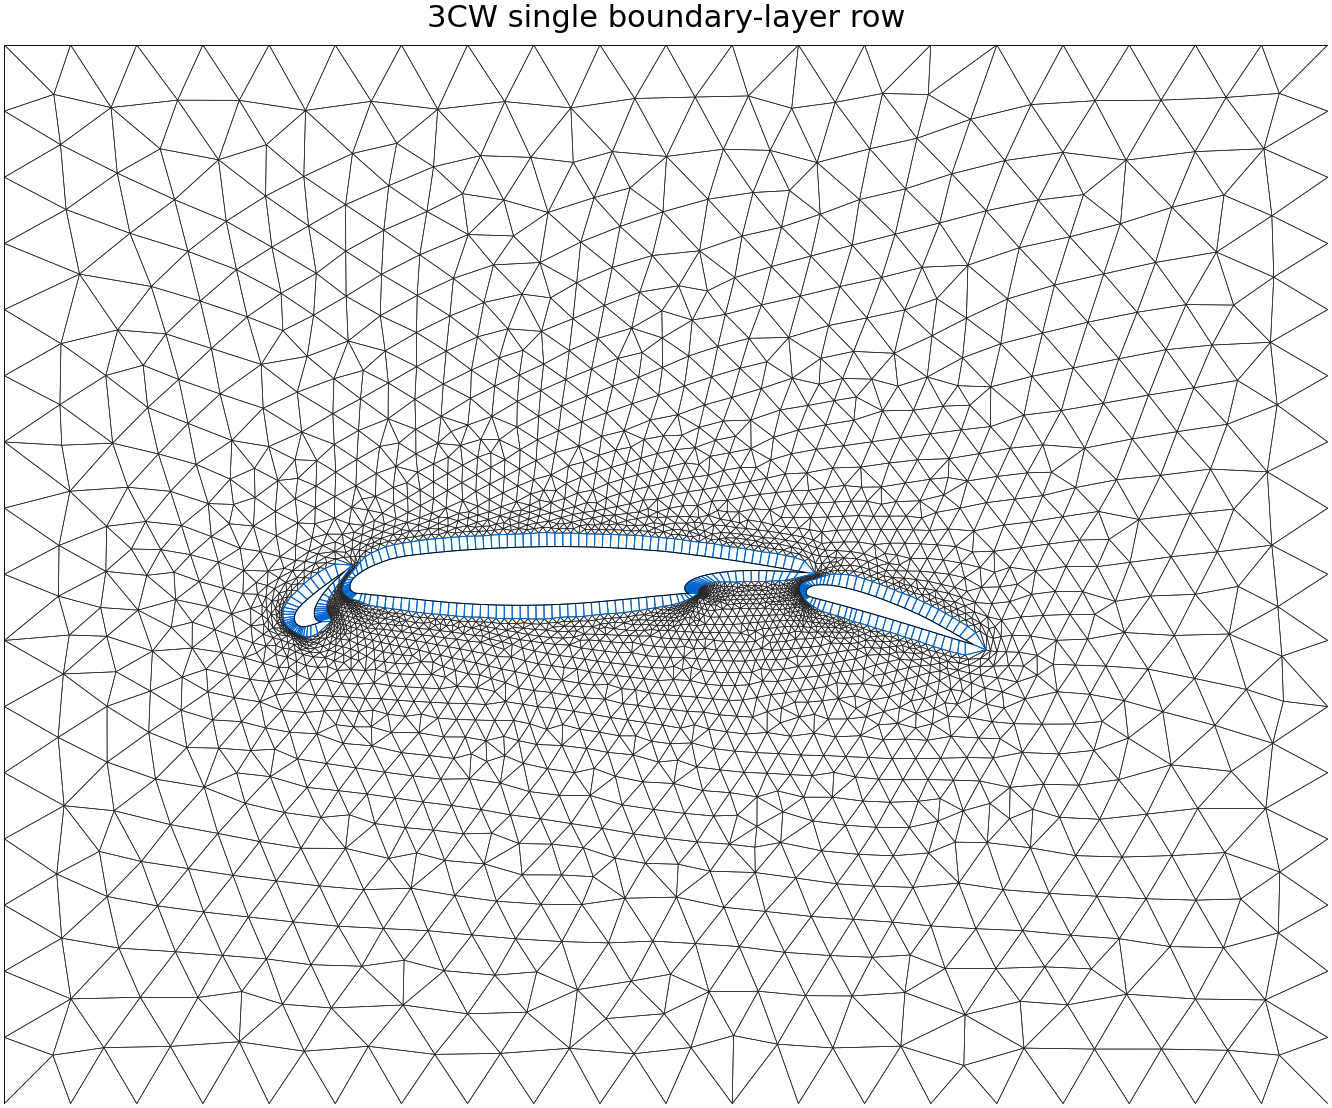
\includegraphics[width=0.82\linewidth]{../figures/3cw_bl_single_layer.png}
\caption{A single boundary-layer row on the 3CW benchmark,
obtained with \(\texttt{Size}=\texttt{Thickness}=40\).}
\label{fig:3cw-first-quad}
\end{figure}

The high-order construction is also inspected before the parametric splitting
of the large layer elements. This exposes the curved \(P_2\) representation
used by the final split mesh, and gives a direct check that the leading and
trailing edges are curved before the layer is subdivided into the requested
graded rows.

\begin{figure}[htbp]
\centering
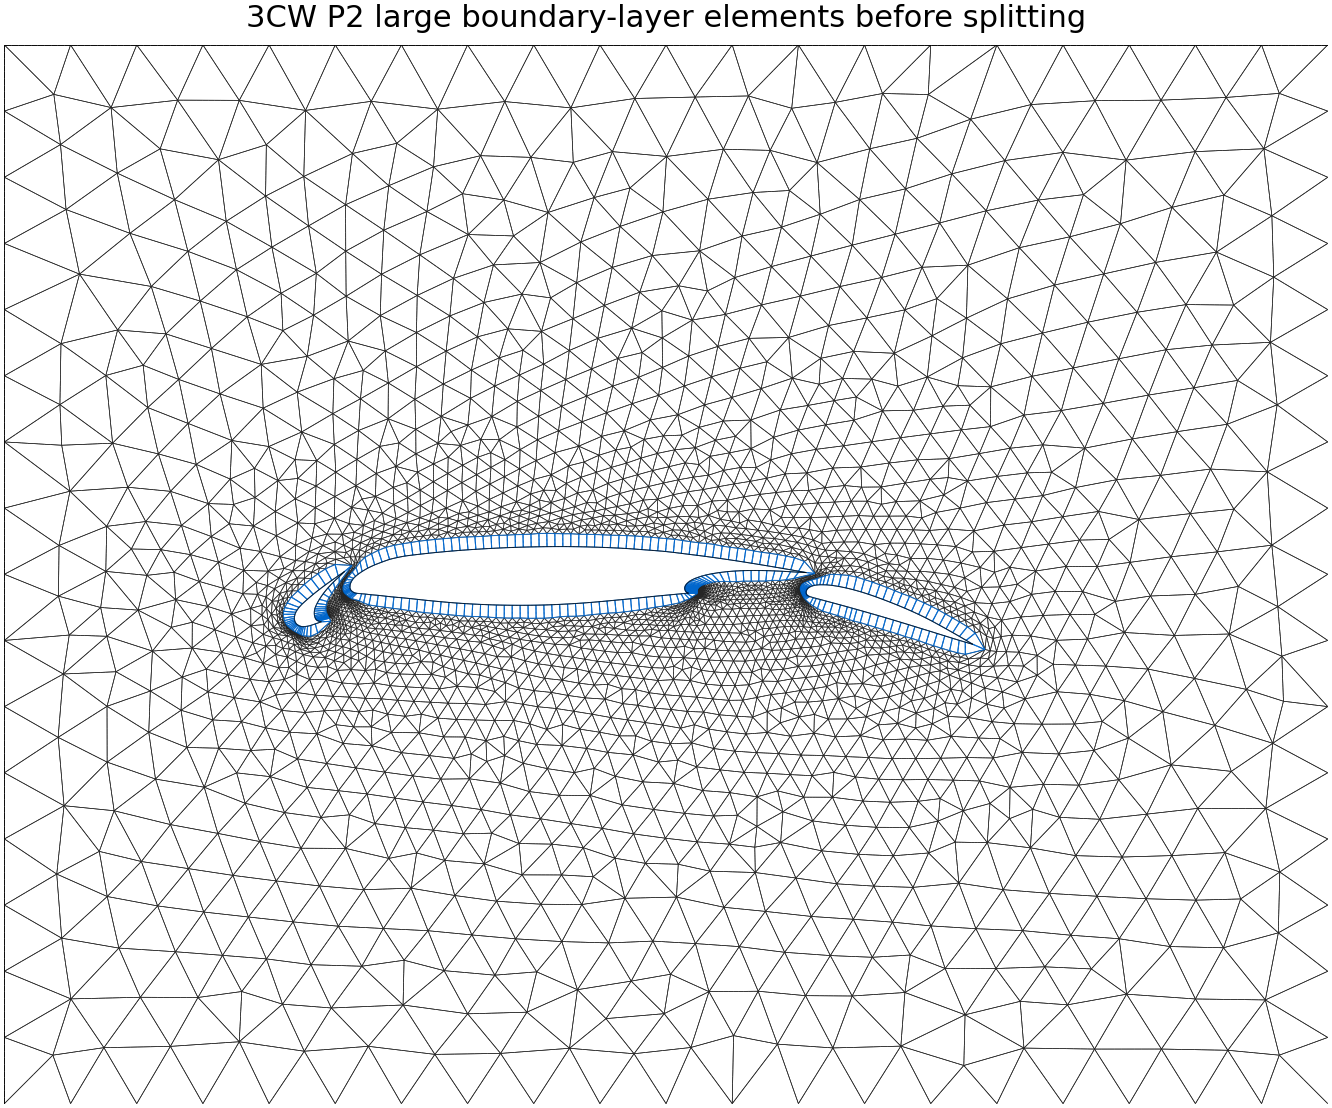
\includegraphics[width=0.82\linewidth]{../figures/3cw_bl_p2_unsplit.png}
\caption{A single \(P_2\) boundary-layer row before parametric splitting. The
large curved quadrangles span the full requested layer thickness before being
split into the final graded sequence.}
\label{fig:3cw-p2-unsplit}
\end{figure}

\begin{figure}[htbp]
\centering
\begin{minipage}{0.48\linewidth}
  \centering
  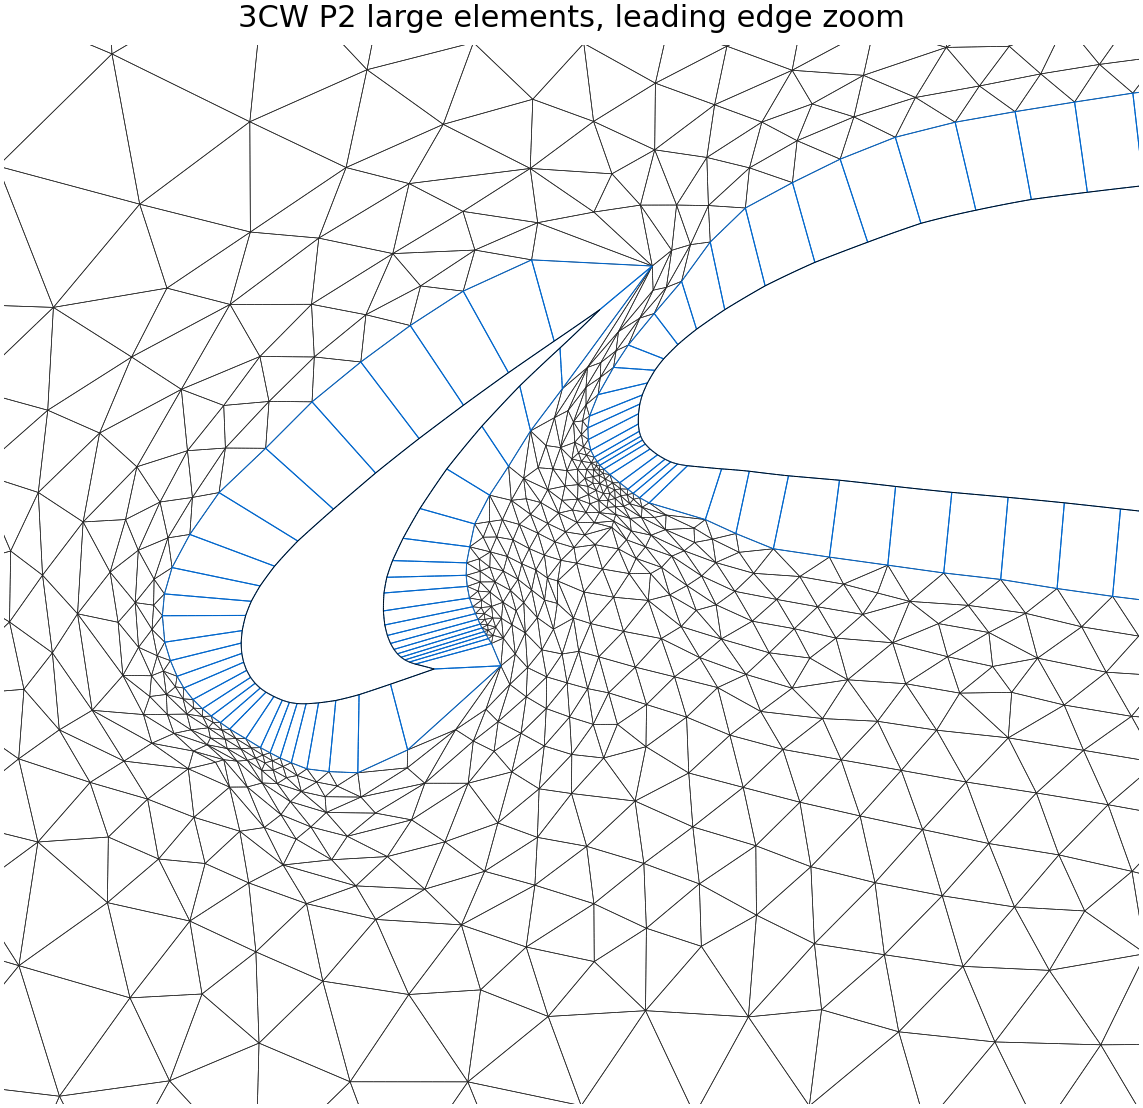
\includegraphics[width=\linewidth]{../figures/3cw_bl_p2_unsplit_leading_edge.png}
\end{minipage}
\hfill
\begin{minipage}{0.48\linewidth}
  \centering
  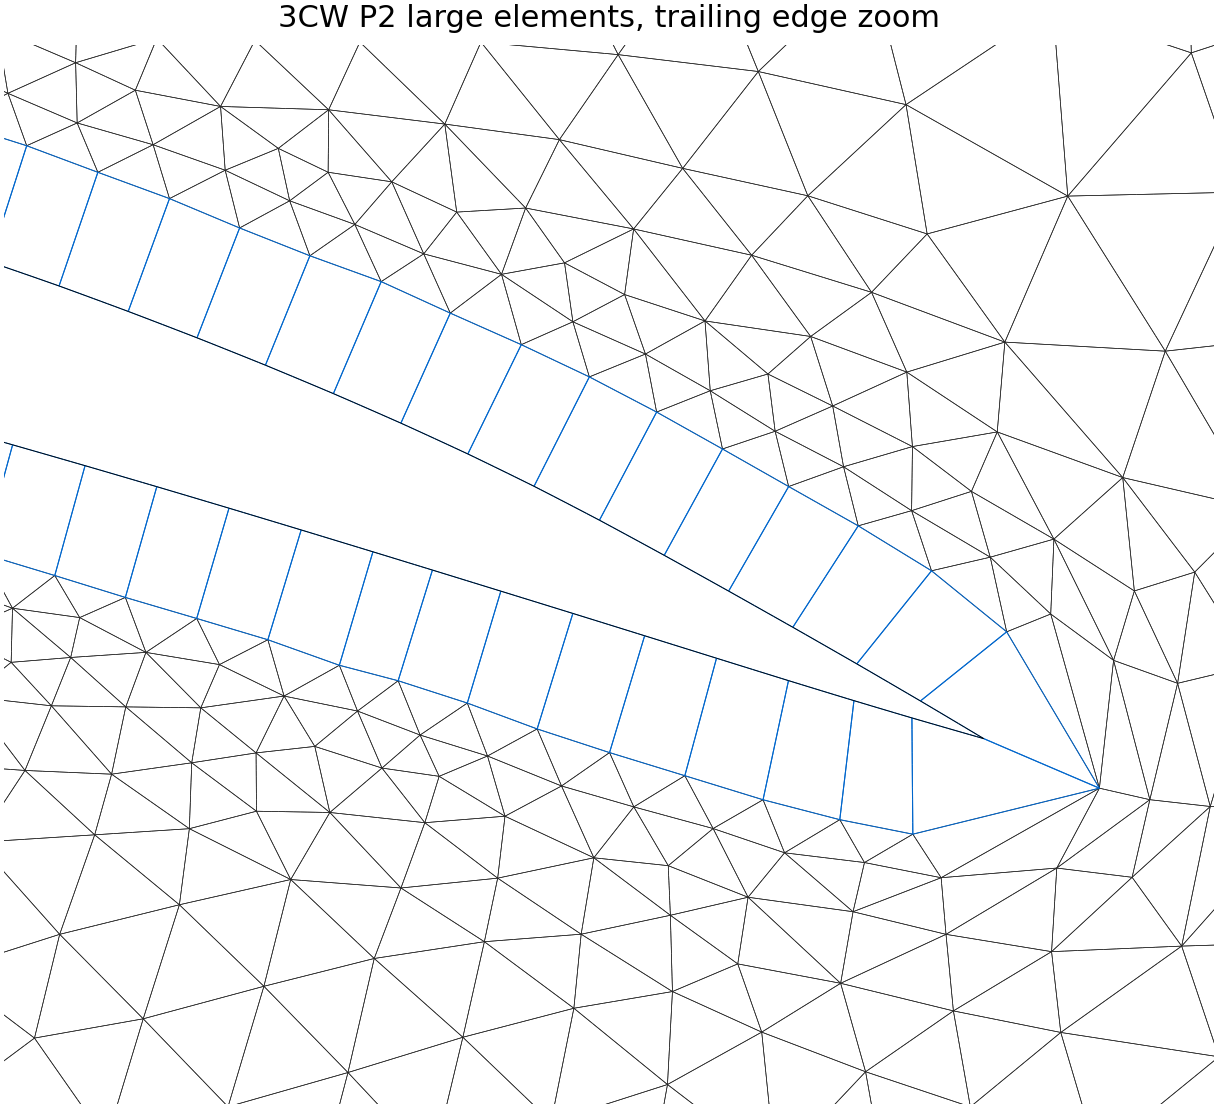
\includegraphics[width=\linewidth]{../figures/3cw_bl_p2_unsplit_trailing_edge.png}
\end{minipage}
\caption{Large \(P_2\) boundary-layer elements before parametric splitting,
zoomed near the leading and trailing edges.}
\label{fig:3cw-p2-unsplit-zooms}
\end{figure}

For the final graded boundary layer, the first layer size is \(h_0=0.3\), and
the geometric growth factor is
\(r=1.5\). The layer sequence generated before exceeding the requested
thickness is
\[
  0.3,\ 0.45,\ 0.675,\ 1.0125,\ 1.51875,\ 2.278125,\ 3.4171875,\
  5.12578125,\ 7.688671875,\ 11.5330078125,
\]
with cumulative thickness
\[
  H = 33.9990234375.
\]
Thus the layer contains ten quadrilateral rows. In the test run, the 189
quadrangles created along the wall were split into \(189\times10=1890\)
high-order layer quadrangles.

\begin{center}
\begin{tabular}{l|r}
Quantity & Value \\
\hline
Initial surface mesh & 1397 vertices, 2846 triangles \\
Boundary-layer support & surface 16, curves 1--7 \\
Mesh size factor for figures & 0.5 \\
Layer rows & 10 \\
Wall quadrangles before splitting & 189 \\
Layer quadrangles after splitting & 1890 \\
Single-row batch time & 0.089 s \\
\(P_2\) large-element batch time & 0.227 s \\
Final split \(P_2\) batch time & 0.273 s \\
Final split \(P_2\), global smoothing batch time & 0.533 s
\end{tabular}
\end{center}

\begin{figure}[htbp]
\centering
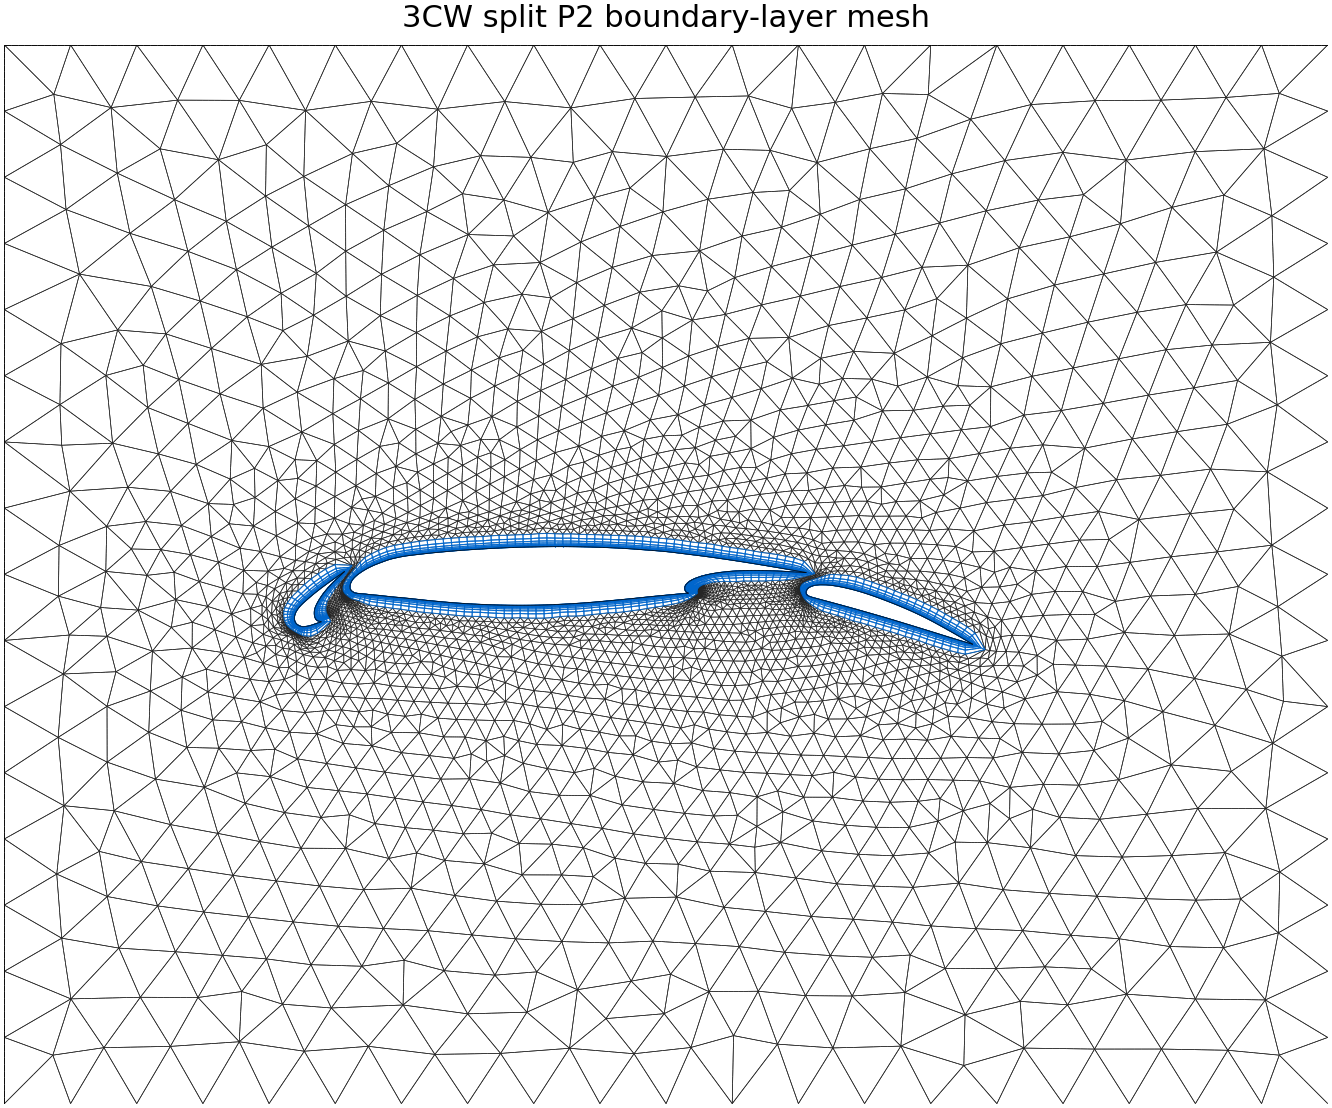
\includegraphics[width=0.82\linewidth]{../figures/3cw_bl.png}
\caption{Final \(P_2\) boundary-layer mesh generated on the 3CW benchmark,
after splitting the large curved layer elements into ten graded rows. The wall
curves 1--7 support the layer; the rest of the surface mesh is preserved and
adjusted by the smoothing/untangling stage.}
\label{fig:3cw-bl}
\end{figure}

\begin{figure}[htbp]
\centering
\begin{minipage}{0.48\linewidth}
  \centering
  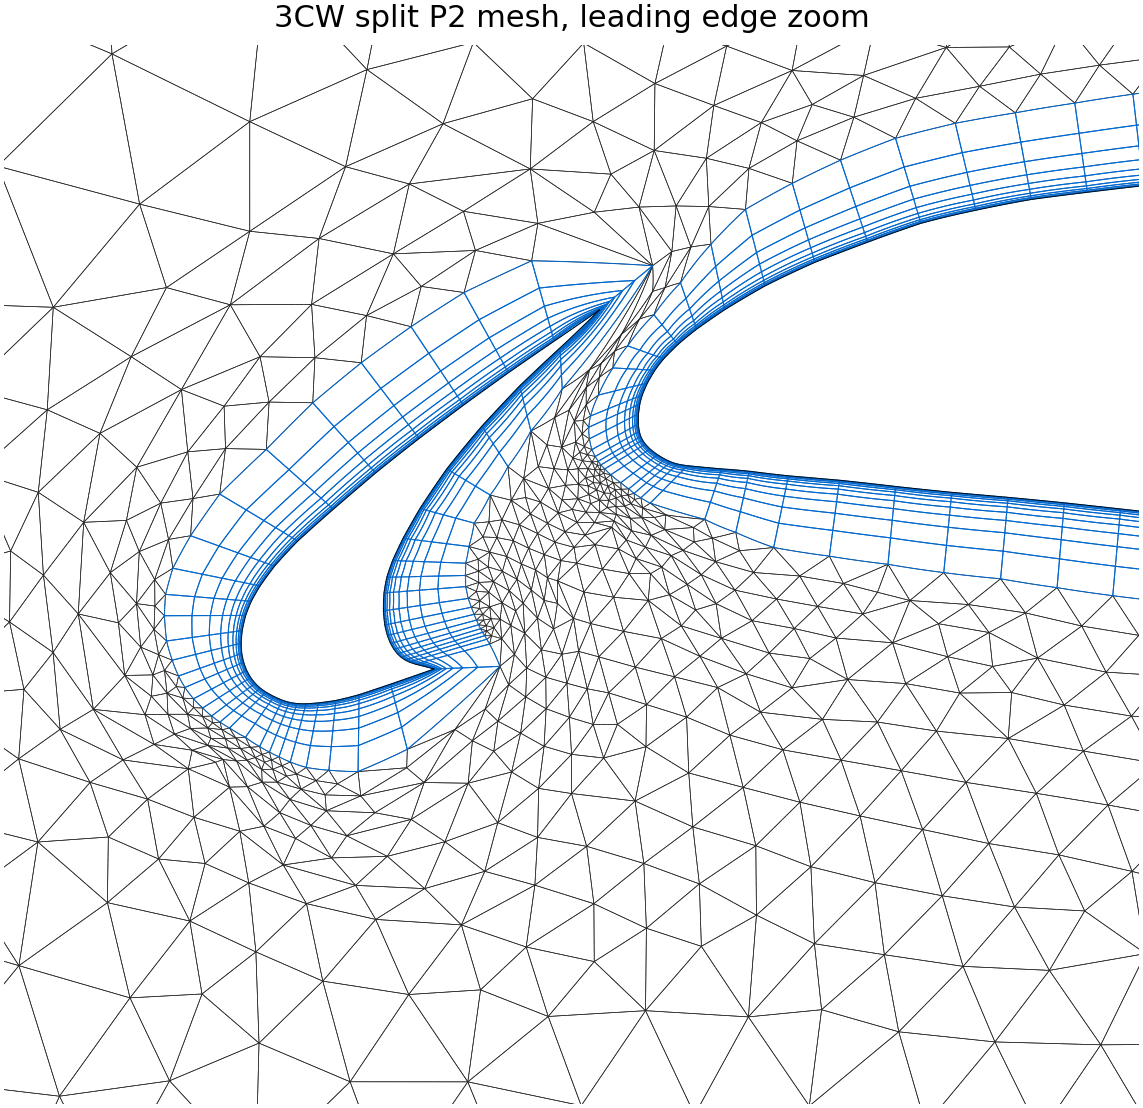
\includegraphics[width=\linewidth]{../figures/3cw_bl_leading_edge.png}
\end{minipage}
\hfill
\begin{minipage}{0.48\linewidth}
  \centering
  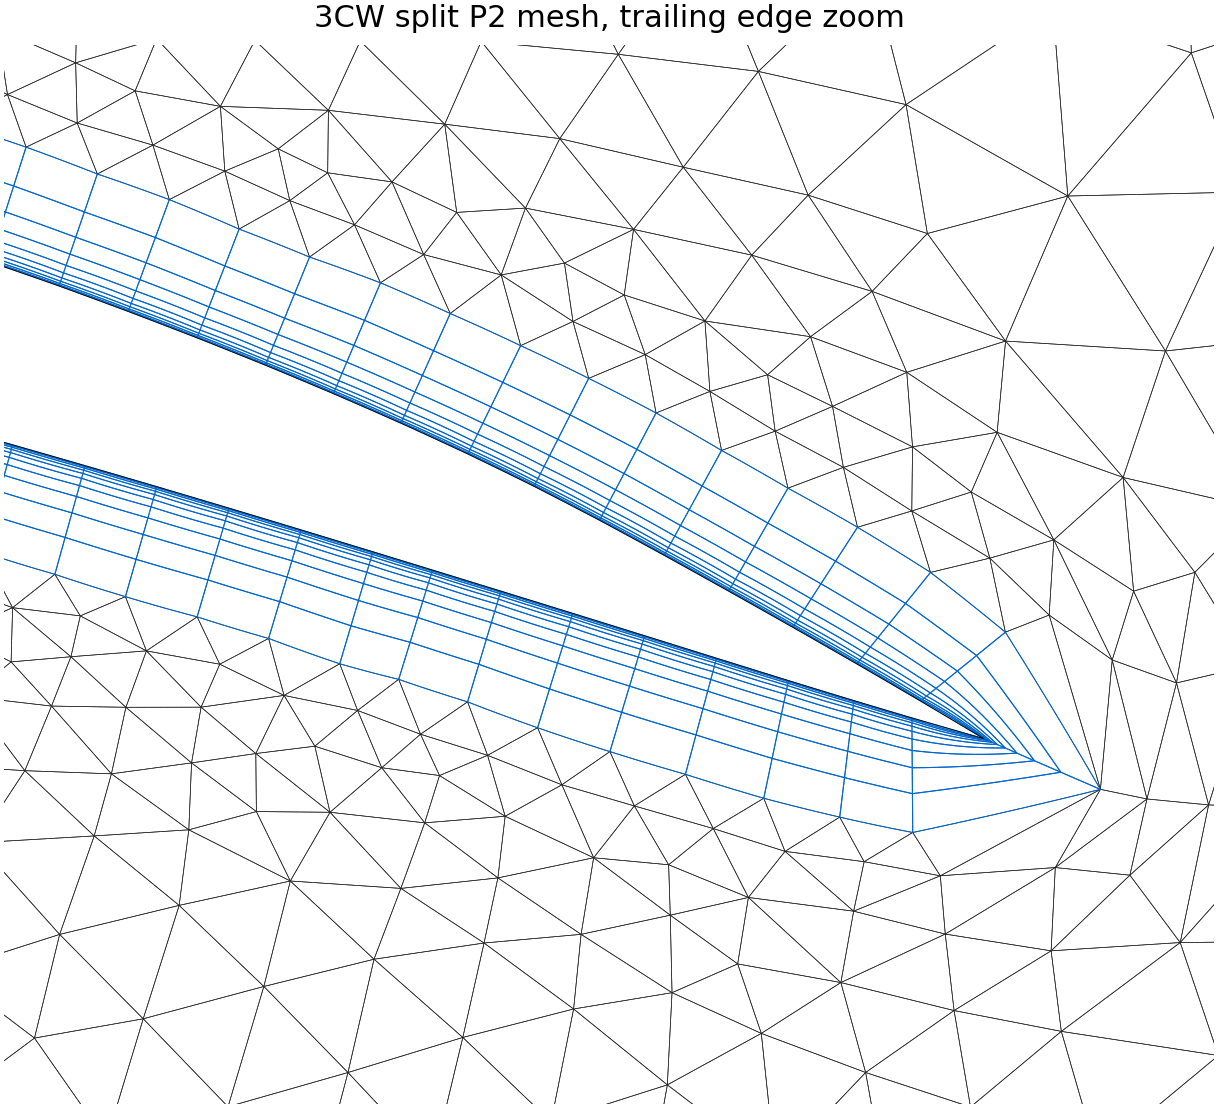
\includegraphics[width=\linewidth]{../figures/3cw_bl_trailing_edge.png}
\end{minipage}
\caption{Zooms near the leading and trailing edges of the 3CW boundary-layer
mesh. The blue quadrangles are the inserted boundary-layer cells.}
\label{fig:3cw-edge-zooms}
\end{figure}

The same split \(P_2\) mesh can be smoothed over a much larger neighborhood by
increasing the number of smoothing rings. For illustration,
\(\texttt{SmoothingLayers}=100\) produces the global adjustment shown in
Fig.~\ref{fig:3cw-global-smoothing}. This is more expensive than the local
setting used in the previous figures, but it remains inexpensive on this
example and propagates the displacement farther into the background mesh.

\begin{figure}[htbp]
\centering
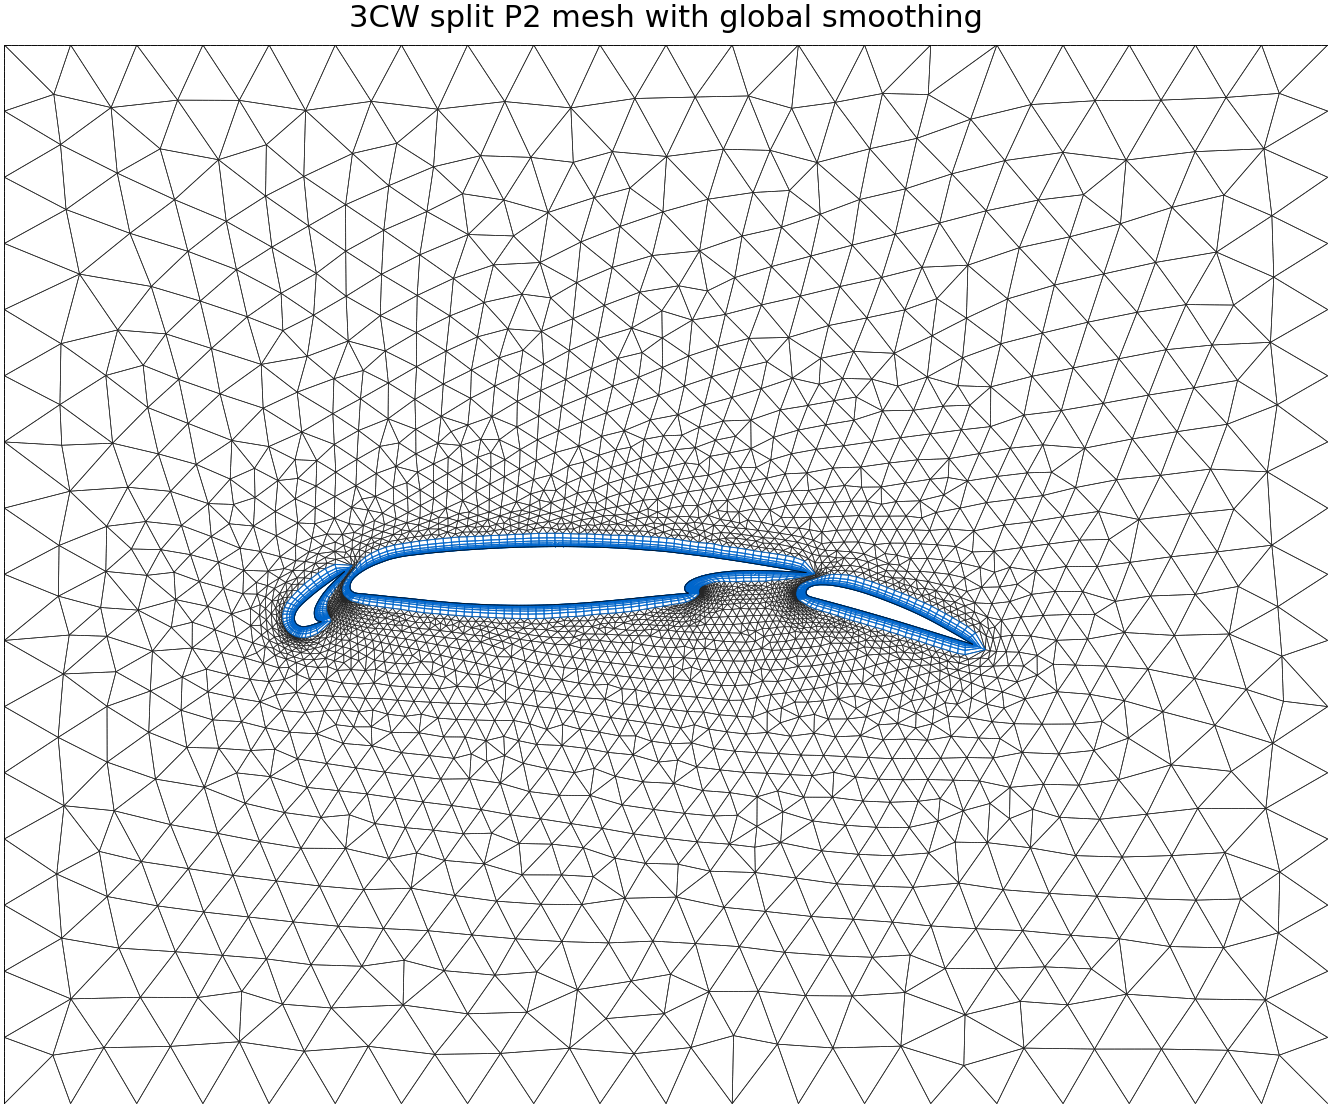
\includegraphics[width=0.82\linewidth]{../figures/3cw_bl_global_smoothing.png}
\caption{Final split \(P_2\) boundary-layer mesh with global smoothing
(\(\texttt{SmoothingLayers}=100\)).}
\label{fig:3cw-global-smoothing}
\end{figure}

\begin{figure}[htbp]
\centering
\begin{minipage}{0.48\linewidth}
  \centering
  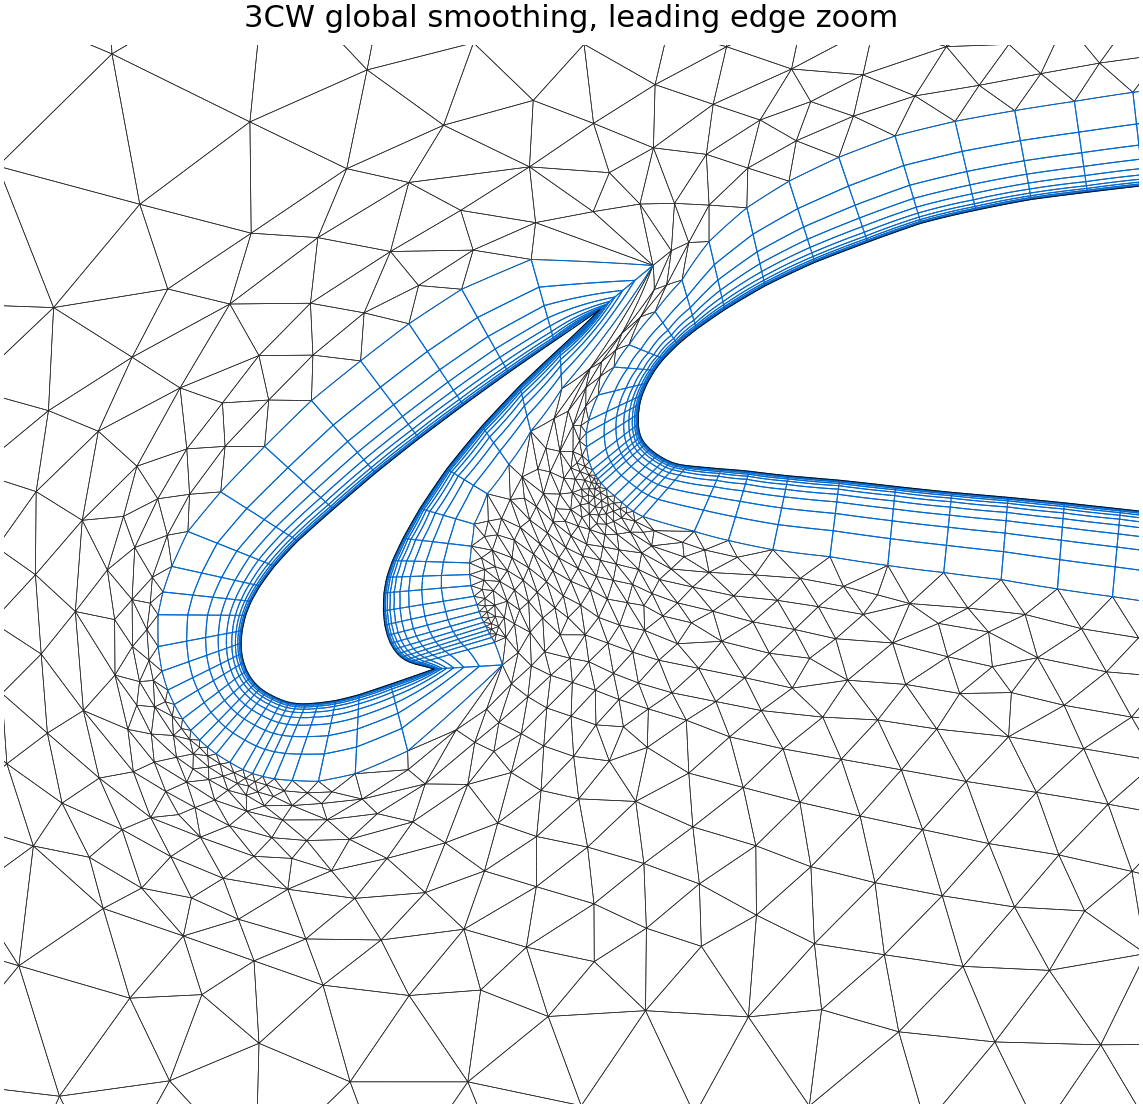
\includegraphics[width=\linewidth]{../figures/3cw_bl_global_smoothing_leading_edge.png}
\end{minipage}
\hfill
\begin{minipage}{0.48\linewidth}
  \centering
  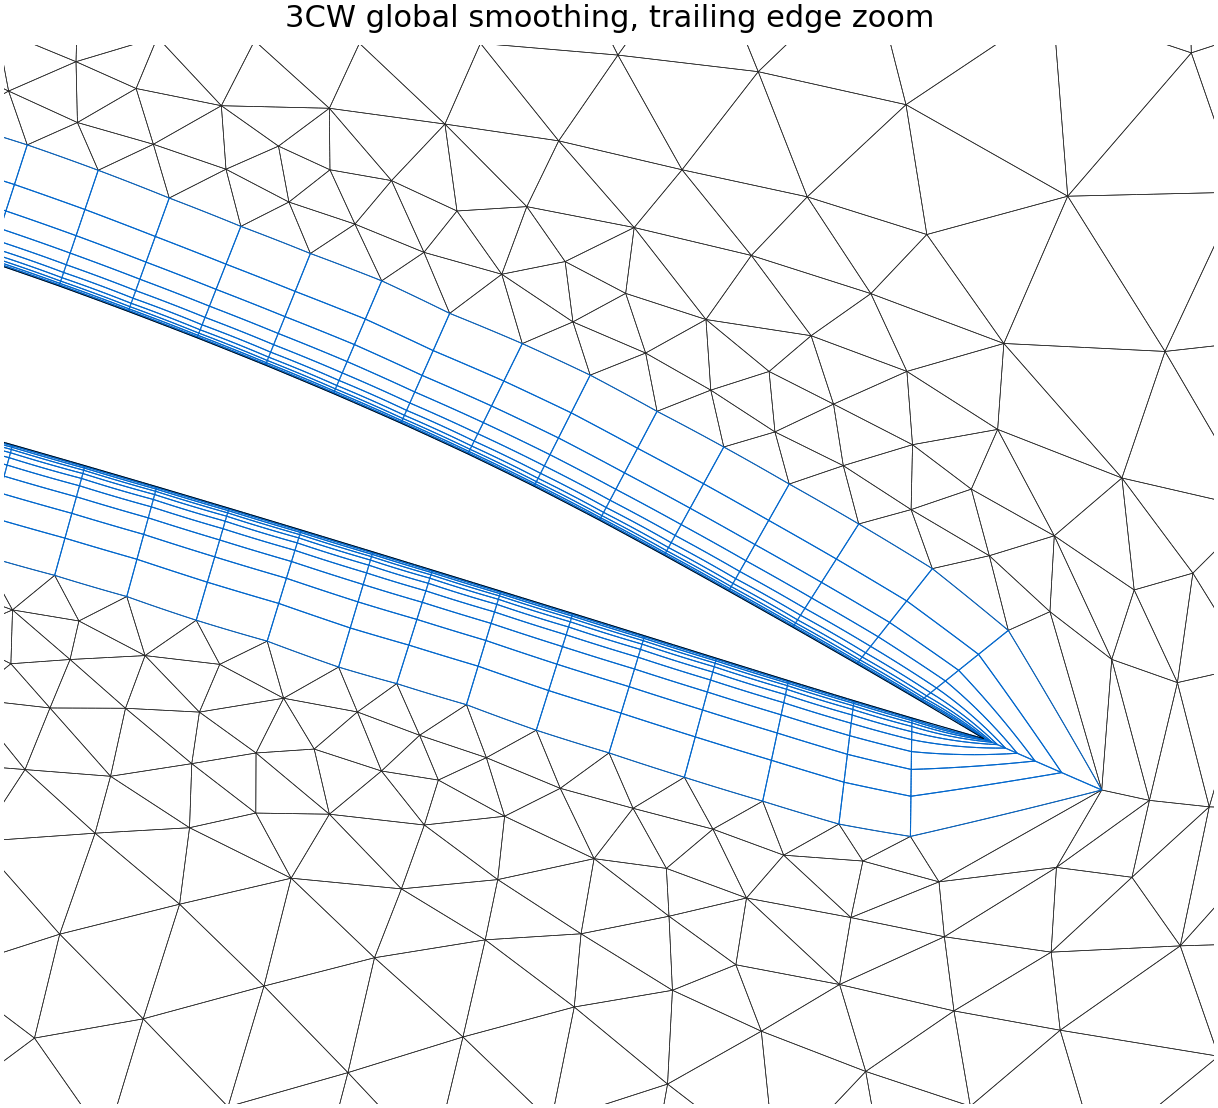
\includegraphics[width=\linewidth]{../figures/3cw_bl_global_smoothing_trailing_edge.png}
\end{minipage}
\caption{Zooms near the leading and trailing edges for the globally smoothed
split \(P_2\) boundary-layer mesh.}
\label{fig:3cw-global-smoothing-zooms}
\end{figure}

To check that the layer has actually been pushed through the mesh, we traversed
the quadrilateral layer chains starting from each mesh edge on curves 1 to 7.
All 189 wall edges generate exactly ten quadrilateral layers. The measured
distance between the wall edge midpoint and the outer layer edge midpoint was
\[
  \min = 10.52,\qquad
  \text{average} = 28.79,\qquad
  \max = 33.02.
\]
The final displacement is of the same order as the cumulative target thickness,
but local values vary because the mesh is constrained by the surrounding
triangulation and by the untangling step. The construction should therefore be
understood as follows: the first layers are placed according to the requested
geometric progression and preserve the boundary-layer scale near the wall;
farther away from the wall, the algorithm does the best possible adjustment to
reconnect smoothly to the existing mesh without breaking its topology.

With the global smoothing setting, the same measurement gives
\[
  \min = 10.34,\qquad
  \text{average} = 33.06,\qquad
  \max = 37.55,
\]
which is closer to the cumulative target thickness \(H=33.9990234375\).

\subsection{Example: RAE2822 Transonic Airfoil}

As a second test, we consider a classical RAE2822 transonic airfoil case. The
calculation shown here uses
\[
  M_\infty = 0.734,\qquad
  \alpha = 2.8^\circ,\qquad
  Re = 6.5\times 10^6.
\]
The mesh is generated by the boundary-layer plugin from the existing
two-dimensional airfoil mesh. In this run we deliberately use the mesh field
defined in the input geometry file as-is: no additional shock-aligned
refinement is added by the post-processing script. The purpose is to check that
the boundary-layer mesh can be used directly in a standard RANS workflow.

The generated mesh contains 9886 grid points and 14664 elements, including
9855 triangles and 4809 quadrangles. The first cell height used at the wall is
\(2\times 10^{-5}\), with a total requested boundary-layer thickness of
\(5\times 10^{-3}\). The final surface \(y^+\) values obtained by SU2 are
between 0.21 and 8.30, with an average value of 4.23 on the airfoil.

\begin{figure}[htbp]
\centering
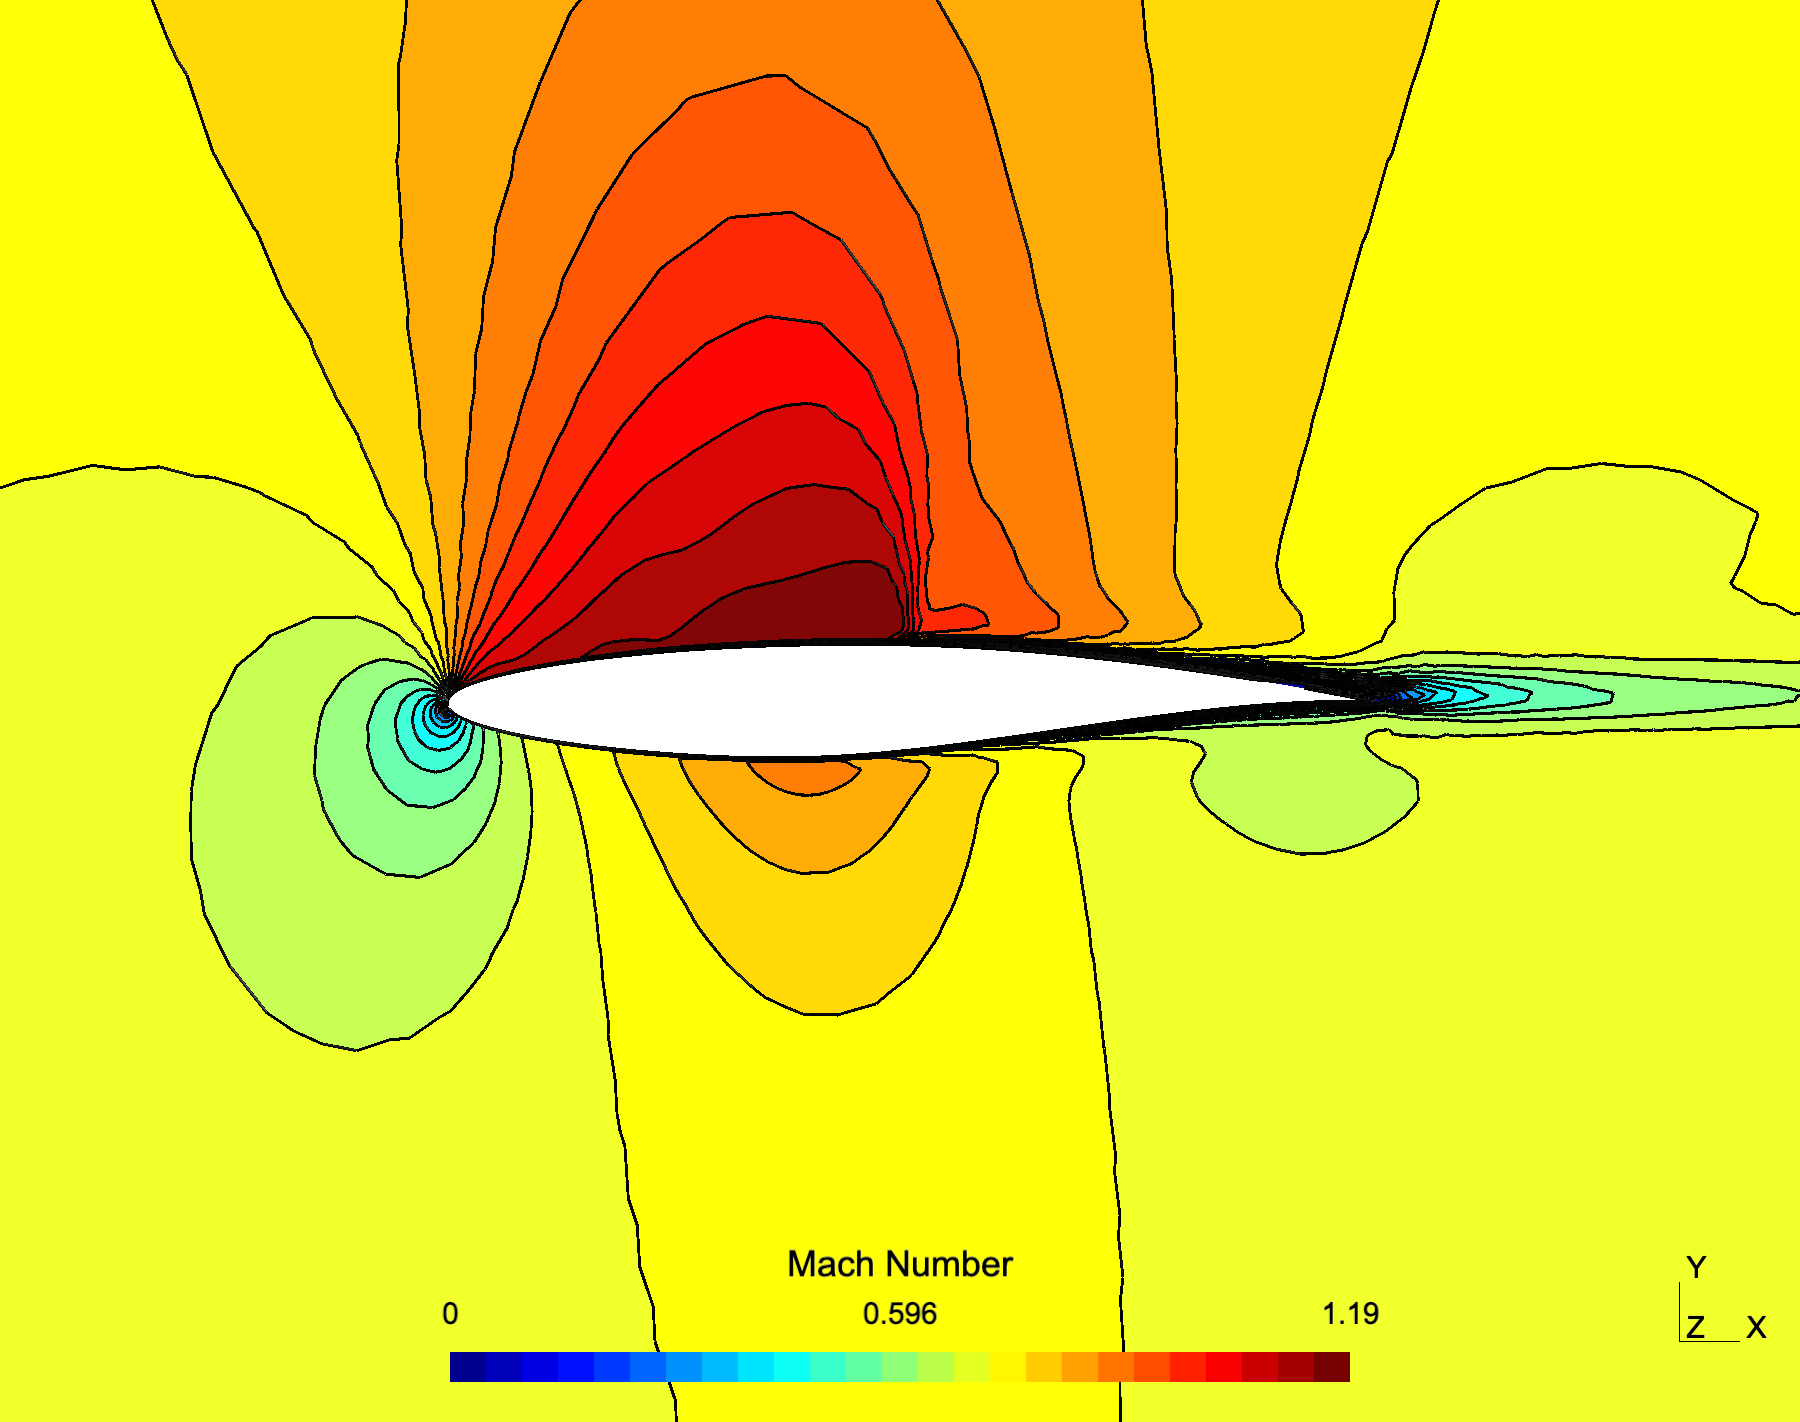
\includegraphics[width=0.6\linewidth]{../figures/rae2822_mach.png}
\caption{Mach number field for the RAE2822 RANS computation on the generated
boundary-layer mesh. The maximum Mach number in this preliminary run is
approximately 1.19.}
\label{fig:rae2822-mach}
\end{figure}

\begin{figure}[htbp]
\centering
\begin{minipage}{0.48\linewidth}
  \centering
  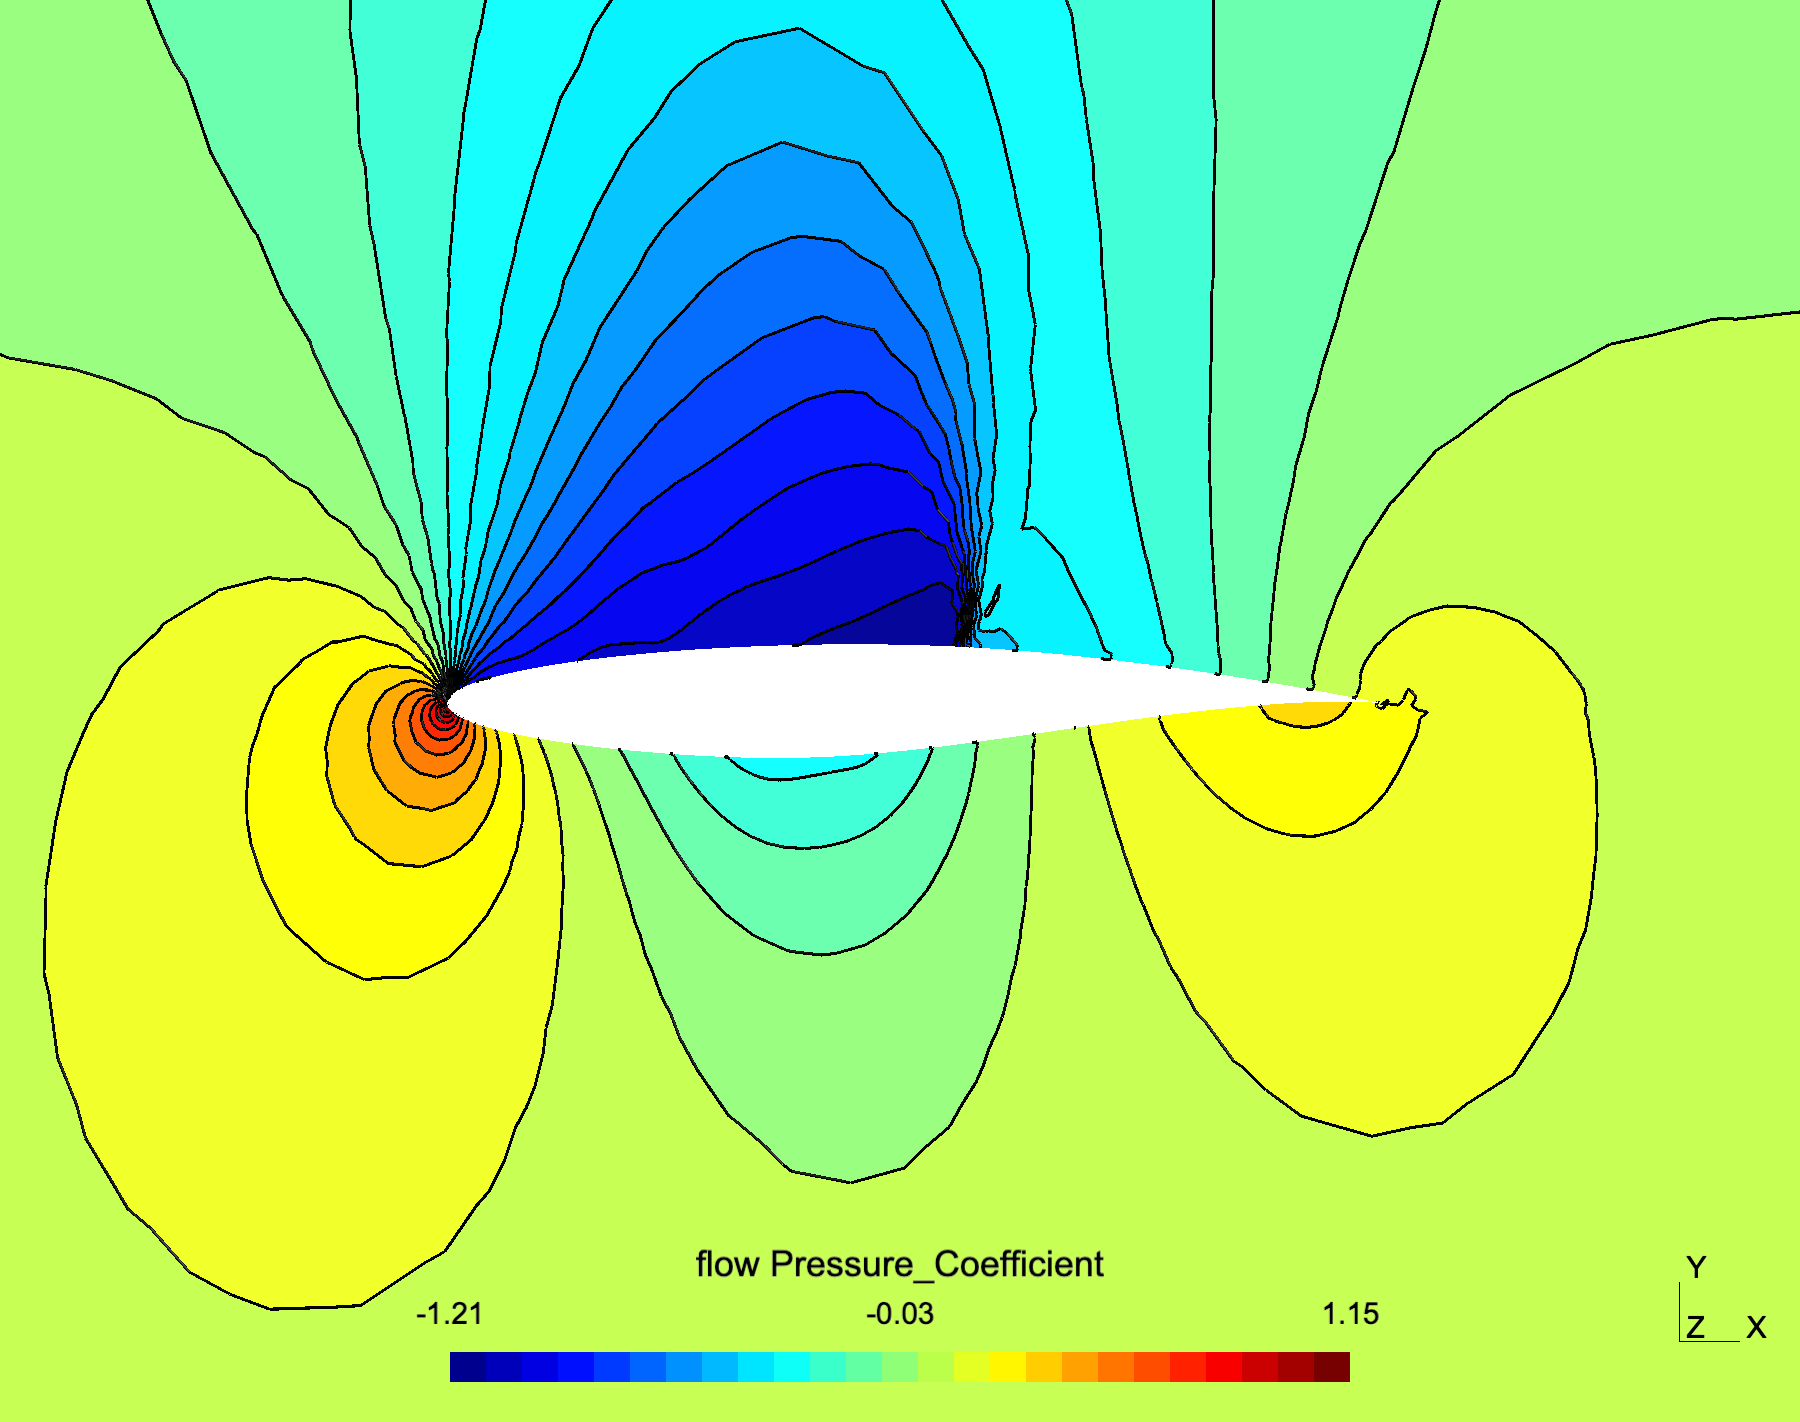
\includegraphics[width=\linewidth]{../figures/rae2822_cp.png}
\end{minipage}
\hfill
\begin{minipage}{0.48\linewidth}
  \centering
  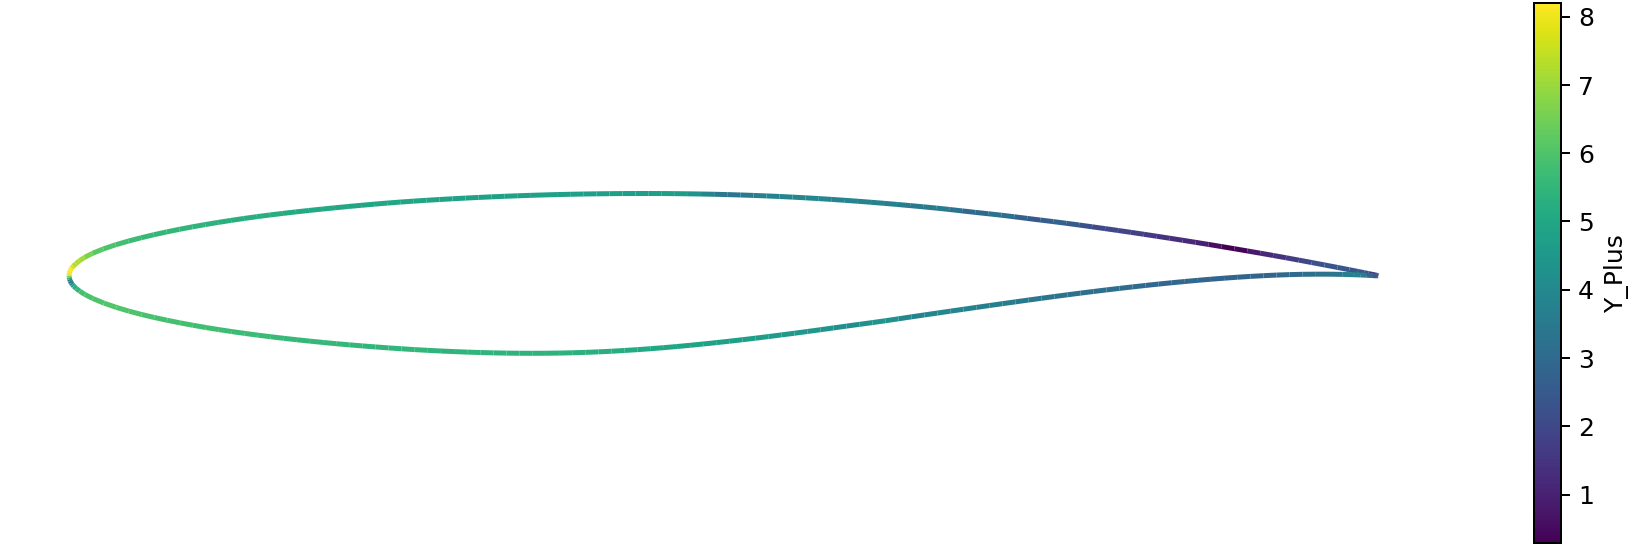
\includegraphics[width=\linewidth]{../figures/rae2822_surface_yplus.png}
\end{minipage}
\caption{Pressure coefficient in the computational domain, and wall \(y^+\) on
the airfoil for the RAE2822 calculation.}
\label{fig:rae2822-cp-yplus}
\end{figure}

The computation was restarted from the first run and continued until the
density residual reached \(10^{-8}\). The final integrated coefficients are
stable, but the lift remains lower than the commonly quoted experimental value,
which indicates that the present setup should still be regarded as a
mesh/solver sanity check rather than a validated aerodynamic computation.
Table~\ref{tab:rae2822-clcd} compares the present computation with the
commonly quoted
experimental reference values for the RAE2822 transonic case at
\(M_\infty=0.734\), \(\alpha\simeq 2.8^\circ\) and \(Re=6.5\times 10^6\).

\begin{table}[htbp]
\centering
\begin{tabular}{l|c|c}
Case & \(C_L\) & \(C_D\) \\
\hline
Experiment, RAE2822 reference case & 0.803 & 0.0168 \\
Present SU2 run on the boundary-layer mesh & 0.637 & 0.0191
\end{tabular}
\caption{Lift and drag comparison for the RAE2822 test case. The
present values are intended as a mesh/solver sanity check, not as a fully
grid-converged validation computation.}
\label{tab:rae2822-clcd}
\end{table}

\subsection{Zero-Thickness Elements}

The first internal stage of the boundary-layer plugin is purely topological. No
optimization is performed at this point, and no point is displaced away from the
initial mesh. The purpose of this stage is to create a set of flat,
zero-thickness boundary-layer elements with the correct connectivity. The
subsequent smoothing, untangling and splitting steps can then move these nodes
without having to repair the topology.

The central data structure is a map
\[
  \texttt{spawned} : MVertex^\star \mapsto
  \{MVertex^\star_1,MVertex^\star_2,\ldots\},
\]
which associates an existing mesh vertex with the copies that have been created
on adjacent model entities. These copies initially have the same physical
coordinates as the original vertex, but they are classified on the entity into
which the boundary layer will grow: a face in two dimensions, or a region in
three dimensions. The classification is essential. It tells the rest of the mesh
which copy should be used on each side of the future layer.

\subsection{Two-Dimensional Boundary Layers}

In two dimensions the user specifies a set of faces where the mesh will be
modified and a set of curves from which the boundary layer will be grown. The
algorithm proceeds as follows.

\begin{enumerate}
  \item The plugin first visits all model vertices incident to the selected
  boundary-layer curves. If all curves incident to such a model vertex belong to
  the boundary layer, a copy of the corresponding mesh vertex is created on each
  selected face adjacent to that point. If only some incident curves belong to
  the boundary layer, copies are instead inserted on the adjacent curves that do
  not belong to the layer. This splits the adjacent mesh lines and creates the
  correct ``side'' vertices for the future layer termination.

  \item The plugin then visits all mesh vertices classified on selected
  boundary-layer curves. For every selected adjacent face, it creates a
  coincident face vertex with the same physical coordinates and stores it in the
  \texttt{spawned} map.

  \item Existing surface elements in the selected faces are reconnected to the
  spawned copies whenever such copies are classified on the face, or on one of
  its boundary curves. Thus the old surface mesh is not duplicated blindly: each
  triangle or quadrangle is made to use the vertex copy that belongs to its side
  of the future layer.

  \item Finally, for every mesh line on a selected boundary-layer curve, the
  plugin creates one zero-thickness quadrangle. Its two first vertices are the
  original line vertices on the wall curve. Its two other vertices are the
  spawned copies used by the adjacent surface mesh. The code searches the edge
  already present in the adjacent surface elements and uses its orientation to
  choose the quadrangle ordering. This is the local check that prevents the
  layer element from being connected with the wrong orientation.
\end{enumerate}

At the end of this process the layer consists of quadrangles whose two opposite
edges coincide geometrically. They are nevertheless valid topological entities:
one edge belongs to the boundary curve and the other edge belongs to the
interior copy used by the surface mesh. Each created quadrangle is stored in the
\texttt{layers} map together with the total layer thickness that will be used by
the later expansion step.

\subsection{Three-Dimensional Boundary Layers}

In three dimensions the user specifies a set of volumes and a set of faces from
which the boundary layer has to be grown. The same principle is applied one
dimension higher. The selected faces form the support of the layer; the selected
regions are the volumes into which the layer is inserted.

The plugin first creates coincident copies of all mesh vertices that must be
separated topologically. Mesh vertices classified on selected faces are copied
into the selected adjacent regions. Mesh vertices classified on curves and
points are copied either into the selected regions or onto adjacent non-layer
faces and curves, depending on which side of the future boundary layer uses
them. These copies are again recorded in the \texttt{spawned} map.

The existing volume mesh is then reconnected to the spawned region vertices.
This is the key operation: the old tetrahedra, prisms, pyramids or hexahedra
touching the selected wall no longer use the wall vertices themselves, but their
coincident region copies. The wall mesh and the volume mesh are therefore
separated topologically while still occupying the same physical position.

The flat volume layer is then created from the surface mesh on the selected
faces:
\[
  \text{triangle} \longrightarrow \text{prism}, \qquad
  \text{quadrangle} \longrightarrow \text{hexahedron}.
\]
For the corresponding triangular face of the adjacent volume element, ordered
as it appears in the closure of this volume element, let
\((v_0,v_1,v_2)\) be its vertices and
\((\hat v_0,\hat v_1,\hat v_2)\) the spawned copies used by the adjacent
region. The plugin creates the degenerate prism
\[
  (v_0,v_1,v_2,\hat v_0,\hat v_1,\hat v_2).
\]
For the corresponding quadrangular face of the adjacent volume element, with
the same volume-face ordering, it similarly creates the degenerate hexahedron
\[
  (v_0,v_1,v_2,v_3,\hat v_0,\hat v_1,\hat v_2,\hat v_3).
\]
All these elements have zero geometric thickness at creation time, because
\(v_i\) and \(\hat v_i\) have identical coordinates. Their topology is however
already the topology of the final boundary-layer volume mesh.

The same mechanism is used on adjacent side faces. When a boundary-layer curve
is shared by a selected wall face and another face of the same volume, the code
creates the necessary spawned vertices on that side face, reconnects the side
surface mesh to them, and inserts the corresponding zero-thickness side
quadrangles. These side faces are stored for the later surface expansion. This
keeps the volume layer watertight: a side face and the prisms or hexahedra that
use it share the same vertex pointers, not merely the same coordinates.

Embedded curves and embedded faces are handled with the same rule, but with an
additional side classification. The plugin records, for each embedded entity,
which surface or volume elements lie on each side. It then creates one spawned
copy per side when needed, replaces the vertices of the adjacent elements by the
copy belonging to that side, and creates the zero-thickness elements between the
original entity and the corresponding spawned side entity.

The important invariant is that a mesh vertex is never duplicated without also
recording where the duplicate is classified and which element side should use
it. Boundary-layer elements are always built from an original support entity and
the spawned copies that have already been assigned to the neighboring mesh. This
is what makes the construction robust: before any node is moved, every element
already shares exactly the vertices it should share in the final mesh.

\section{Introduction}

Boundary layer meshes generated on curved CAD surfaces are often constructed by
extruding a surface mesh in a normal direction. Before the volume mesh can be
optimized, the surface mesh supporting the layer must be untangled and smoothed.
For CAD surfaces, a natural strategy is to move vertices in the parametric
domain and project them back to the surface. However, the parametric domain can
be severely distorted even when the corresponding physical surface is almost
planar. Optimizing a mesh directly in that distorted parametric space can then
produce poor physical elements.

The goal of the present method is to keep the optimization variables in the
parametric space, while evaluating the Winslow energy in physical space. This is
done by introducing the first fundamental form of the CAD surface into the
quality functional.

The same construction also provides a practical path to high-order boundary
layers. Once the linear layer has the correct topology and has been pushed into
the mesh, high-order nodes can be inserted consistently on curves, surfaces and
volumes. The curved elements are then treated by inexpensive local checks and
untangling steps based on the same low-order infrastructure. This gives a
high-order boundary-layer mesh that is both robust in practice and cheap enough
for industrial-size meshes.

\section{Surface Parametrization}

Let
\[
  \bx : \Omega \subset \R^2 \rightarrow \R^3,
  \qquad
  (u,v) \mapsto \bx(u,v)
\]
be the CAD surface parametrization. The surface metric, or first fundamental
form, is
\[
  \bG(u,v) =
  \begin{pmatrix}
    \bx_u \cdot \bx_u & \bx_u \cdot \bx_v \\
    \bx_u \cdot \bx_v & \bx_v \cdot \bx_v
  \end{pmatrix}.
\]
The physical area element is
\[
  \dd A = \sqrt{\det \bG(u,v)}\,\dd u\,\dd v.
\]

Consider one mesh triangle whose vertices are represented by parametric
coordinates
\[
  \bu_i = (u_i,v_i), \qquad i=1,2,3.
\]
The corresponding physical vertices are
\[
  \bx_i = \bx(\bu_i).
\]

\section{Ideal Element}

For each surface triangle, we define an ideal triangle in a local two
dimensional coordinate system:
\[
  \bX_i = (\xi_i,\eta_i), \qquad i=1,2,3.
\]
For a boundary-layer element, the ideal element should encode the desired
anisotropy of the layer. For a bulk triangle, it can be chosen to preserve the
physical shape of the original triangle, or to be an equilateral reference
triangle. The only strict convention is that the ideal triangle must have
positive signed area:
\[
  A_I =
  \frac{1}{2}
  \det
  \begin{pmatrix}
    \xi_2-\xi_1 & \xi_3-\xi_1 \\
    \eta_2-\eta_1 & \eta_3-\eta_1
  \end{pmatrix}
  > 0.
\]

The finite element map from ideal coordinates to parametric coordinates is
linear on each triangle:
\[
  \bu(\bX) =
  \sum_{i=1}^3 N_i(\bX)\,\bu_i,
\]
where \(N_i\) are the linear shape functions on the ideal triangle. Its
Jacobian is
\[
  \bJ =
  \frac{\partial (u,v)}{\partial(\xi,\eta)}
  =
  \begin{pmatrix}
    u_\xi & u_\eta \\
    v_\xi & v_\eta
  \end{pmatrix}.
\]

\section{Coordinate Transformations}

The proposed optimization uses three coordinate systems. The ideal element
defines the target shape, the parametric element contains the unknowns of the
optimization, and the CAD surface gives the physical geometry where the quality
is measured.

\begin{figure}[htbp]
\centering
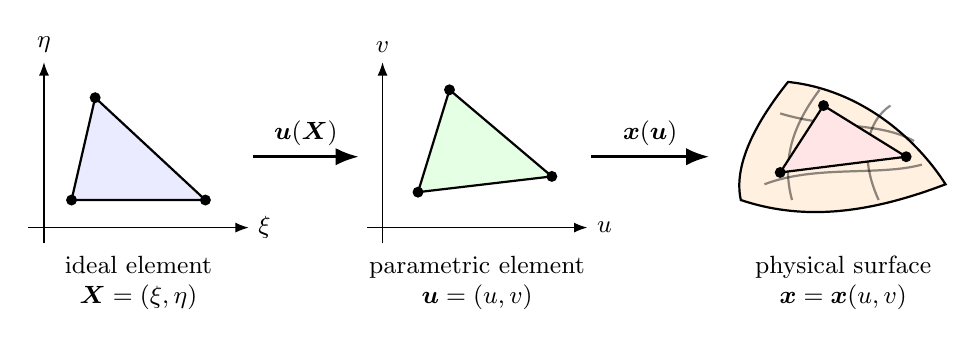
\begin{tikzpicture}[
  >=Latex,
  geom/.style={line width=0.8pt},
  map/.style={->, very thick},
  vertex/.style={circle, fill=black, inner sep=1.4pt},
  label/.style={font=\small}
]
  \begin{scope}[shift={(0,0)}]
    \draw[->] (-0.2,0) -- (2.6,0) node[right,label] {$\xi$};
    \draw[->] (0,-0.2) -- (0,2.1) node[above,label] {$\eta$};
    \coordinate (I1) at (0.35,0.35);
    \coordinate (I2) at (2.05,0.35);
    \coordinate (I3) at (0.65,1.65);
    \draw[geom, fill=blue!8] (I1) -- (I2) -- (I3) -- cycle;
    \foreach \p/\n in {I1/1,I2/2,I3/3}
      \node[vertex, label=below:{\scriptsize $\bX_\n$}] at (\p) {};
    \node[label, align=center] at (1.2,-0.7) {ideal element\\$\bX=(\xi,\eta)$};
  \end{scope}

  \begin{scope}[shift={(4.3,0)}]
    \draw[->] (-0.2,0) -- (2.6,0) node[right,label] {$u$};
    \draw[->] (0,-0.2) -- (0,2.1) node[above,label] {$v$};
    \coordinate (P1) at (0.45,0.45);
    \coordinate (P2) at (2.15,0.65);
    \coordinate (P3) at (0.85,1.75);
    \draw[geom, fill=green!10] (P1) -- (P2) -- (P3) -- cycle;
    \foreach \p/\n in {P1/1,P2/2,P3/3}
      \node[vertex, label=below:{\scriptsize $\bu_\n$}] at (\p) {};
    \node[label, align=center] at (1.2,-0.7) {parametric element\\$\bu=(u,v)$};
  \end{scope}

  \begin{scope}[shift={(8.8,0)}]
    \draw[geom, fill=orange!12]
      (0.05,0.35)
      .. controls (0.8,0.1) and (1.6,0.15) .. (2.65,0.55)
      .. controls (2.3,1.1) and (1.6,1.75) .. (0.65,1.85)
      .. controls (0.25,1.35) and (-0.05,0.8) .. cycle;
    \draw[geom, opacity=0.45]
      (0.35,0.55) .. controls (1.0,0.8) and (1.8,0.65) .. (2.35,0.8);
    \draw[geom, opacity=0.45]
      (0.55,1.45) .. controls (1.2,1.25) and (1.8,1.35) .. (2.25,1.1);
    \draw[geom, opacity=0.45]
      (0.7,0.35) .. controls (0.55,0.9) and (0.75,1.35) .. (1.05,1.75);
    \draw[geom, opacity=0.45]
      (1.8,0.35) .. controls (1.55,0.9) and (1.65,1.35) .. (1.95,1.55);

    \coordinate (X1) at (0.55,0.7);
    \coordinate (X2) at (2.15,0.9);
    \coordinate (X3) at (1.1,1.55);
    \draw[geom, fill=red!10] (X1) -- (X2) -- (X3) -- cycle;
    \foreach \p/\n in {X1/1,X2/2,X3/3}
      \node[vertex, label=above:{\scriptsize $\bx_\n$}] at (\p) {};
    \node[label, align=center] at (1.35,-0.7) {physical surface\\$\bx=\bx(u,v)$};
  \end{scope}

  \draw[map] (2.65,0.9) -- node[above,label] {$\bu(\bX)$} (4.0,0.9);
  \draw[map] (6.95,0.9) -- node[above,label] {$\bx(\bu)$} (8.45,0.9);
\end{tikzpicture}
\caption{Successive coordinate changes. The optimization variables are the
parametric coordinates \(\bu_i\), but the quality is measured after mapping to
the physical surface.}
\label{fig:coordinate-chain}
\end{figure}

At the differential level, an infinitesimal vector in the ideal triangle is
first mapped to the parametric plane by \(\bJ\), then to the tangent plane of
the CAD surface by the surface derivatives \(\bx_u\) and \(\bx_v\).

\begin{figure}[htbp]
\centering
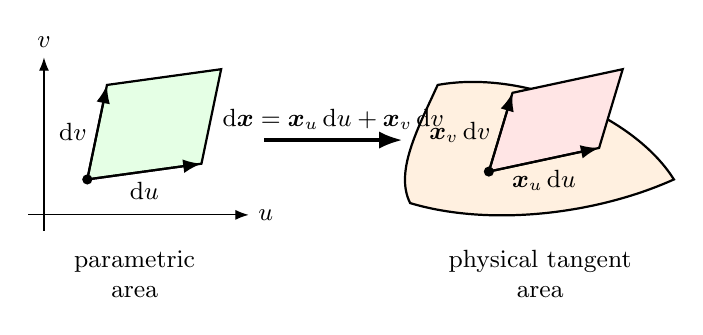
\begin{tikzpicture}[
  >=Latex,
  line/.style={line width=0.8pt},
  map/.style={->, very thick},
  vertex/.style={circle, fill=black, inner sep=1.3pt},
  label/.style={font=\small}
]
  \begin{scope}[shift={(0,0)}]
    \draw[->] (-0.2,0) -- (2.6,0) node[right,label] {$u$};
    \draw[->] (0,-0.2) -- (0,2.0) node[above,label] {$v$};
    \coordinate (O) at (0.55,0.45);
    \coordinate (U) at (2.0,0.65);
    \coordinate (V) at (0.8,1.65);
    \coordinate (UV) at ($(U)+(V)-(O)$);
    \draw[line, fill=green!10] (O) -- (U) -- (UV) -- (V) -- cycle;
    \draw[->, thick] (O) -- node[below,label] {$\dd u$} (U);
    \draw[->, thick] (O) -- node[left,label] {$\dd v$} (V);
    \node[vertex] at (O) {};
    \node[label, align=center] at (1.15,-0.75) {parametric\\area};
  \end{scope}

  \begin{scope}[shift={(5.0,0)}]
    \draw[line, fill=orange!12]
      (-0.35,0.15) .. controls (0.65,-0.15) and (2.0,0.0) .. (3.0,0.45)
      .. controls (2.5,1.25) and (1.1,1.85) .. (0.0,1.65)
      .. controls (-0.25,1.1) and (-0.55,0.55) .. cycle;
    \coordinate (Q) at (0.65,0.55);
    \coordinate (Qu) at (2.05,0.85);
    \coordinate (Qv) at (0.95,1.55);
    \coordinate (Quv) at ($(Qu)+(Qv)-(Q)$);
    \draw[line, fill=red!10] (Q) -- (Qu) -- (Quv) -- (Qv) -- cycle;
    \draw[->, thick] (Q) -- node[below,label] {$\bx_u\,\dd u$} (Qu);
    \draw[->, thick] (Q) -- node[left,label] {$\bx_v\,\dd v$} (Qv);
    \node[vertex] at (Q) {};
    \node[label, align=center] at (1.3,-0.75) {physical tangent\\area};
  \end{scope}

  \draw[map] (2.8,0.95) -- node[above,label] {$\dd\bx=\bx_u\,\dd u+\bx_v\,\dd v$} (4.55,0.95);
\end{tikzpicture}
\caption{The surface metric is the Gram matrix of the tangent vectors:
\(\bG_{ij}=\bx_i\cdot\bx_j\), with \(\bx_1=\bx_u\) and \(\bx_2=\bx_v\).
It converts lengths and areas measured in the parametric plane into physical
surface lengths and areas.}
\label{fig:surface-metric}
\end{figure}

The metric-aware Winslow energy is therefore a standard two-dimensional
Winslow energy applied to the composed map
\[
  \bX
  \xrightarrow{\ \bu(\bX)\ }
  \bu
  \xrightarrow{\ \bx(\bu)\ }
  \bx,
\]
but with the CAD part represented locally by the metric tensor.

\begin{figure}[htbp]
\centering
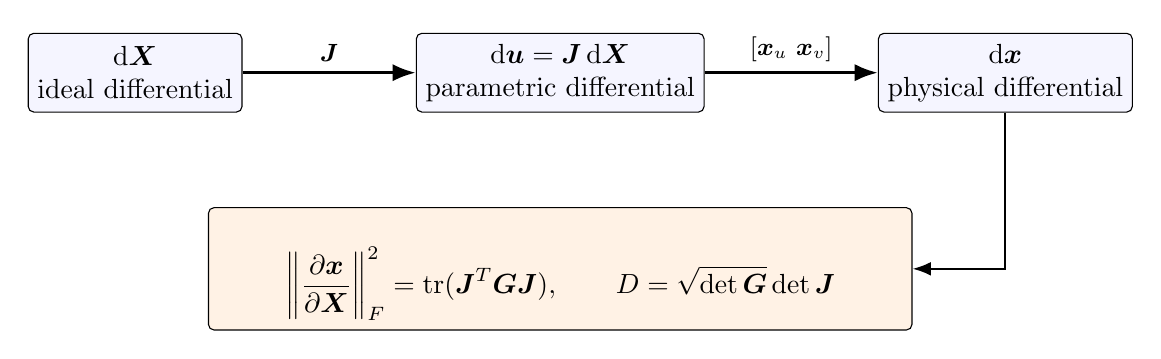
\begin{tikzpicture}[
  >=Latex,
  box/.style={draw, rounded corners=2pt, minimum width=2.7cm,
              minimum height=1.0cm, align=center, fill=blue!4},
  map/.style={->, very thick},
  label/.style={font=\small}
]
  \node[box] (ideal) {$\dd\bX$\\ideal differential};
  \node[box, right=2.2cm of ideal] (param) {$\dd\bu=\bJ\,\dd\bX$\\parametric differential};
  \node[box, right=2.2cm of param] (phys) {$\dd\bx$\\physical differential};

  \draw[map] (ideal) -- node[above,label] {$\bJ$} (param);
  \draw[map] (param) -- node[above,label] {$[\bx_u\ \bx_v]$} (phys);

  \node[draw, fill=orange!10, align=center, below=1.2cm of param,
        rounded corners=2pt, text width=8.7cm] (energy)
  {
    \[
      \left\|\frac{\partial\bx}{\partial\bX}\right\|_F^2
      =
      \operatorname{tr}(\bJ^T\bG\bJ),
      \qquad
      D = \sqrt{\det\bG}\det\bJ
    \]
  };
  \draw[->, thick] (phys.south) |- (energy.east);
\end{tikzpicture}
\caption{Differential composition used in the energy. The optimizer changes
\(\bJ\) through the parametric coordinates, while \(\bG\) accounts for the
physical CAD surface.}
\label{fig:differential-composition}
\end{figure}

\section{Physical Winslow Energy in Parametric Coordinates}

The differential of the physical surface map with respect to ideal coordinates
is
\[
  \frac{\partial \bx}{\partial \bX}
  =
  \frac{\partial \bx}{\partial \bu}
  \frac{\partial \bu}{\partial \bX}.
\]
Consequently, the squared Frobenius norm of the physical Jacobian is
\[
  \left\|
    \frac{\partial \bx}{\partial \bX}
  \right\|_F^2
  =
  \operatorname{tr}\left(\bJ^T \bG \bJ\right).
\]
The physical area scaling between the ideal element and the current curved
surface element is
\[
  D =
  \sqrt{\det \bG}\,\det \bJ.
\]

We use the regularized Winslow energy
\[
  E_T =
  \frac{\operatorname{tr}\left(\bJ^T \bG \bJ\right)}
       {\chi(D)}
  +
  \lambda
  \frac{D^2 + 1}
       {\chi(D)},
\]
with
\[
  \chi(D) =
  \frac{1}{2}\left(D + \sqrt{D^2 + \varepsilon^2}\right).
\]
The derivative of the regularization is
\[
  \chi'(D) =
  \frac{1}{2}
  +
  \frac{D}{2\sqrt{D^2+\varepsilon^2}}.
\]

The total energy is the sum over the triangles:
\[
  E = \sum_{T} A_I\,E_T,
\]
where \(A_I\) is the positive area of the ideal triangle. In practice the
constant factor \(A_I\) can be absorbed in the element contribution if all
ideal gradients are computed with respect to the ideal coordinates.

\section{Element Gradient}

Let
\[
  I = \operatorname{tr}\left(\bJ^T \bG \bJ\right),
  \qquad
  D = \sqrt{\det \bG}\,\det \bJ,
  \qquad
  \chi = \chi(D).
\]
The element energy is
\[
  E_T = \frac{I + \lambda(D^2+1)}{\chi}.
\]
Its derivative with respect to the Jacobian entries is
\[
  \frac{\partial E_T}{\partial \bJ}
  =
  \frac{1}{\chi}
  \frac{\partial I}{\partial \bJ}
  +
  \left(
    \frac{2\lambda D}{\chi}
    -
    \frac{E_T \chi'(D)}{\chi}
  \right)
  \frac{\partial D}{\partial \bJ}.
\]

Writing
\[
  \bG =
  \begin{pmatrix}
    g_{00} & g_{01} \\
    g_{01} & g_{11}
  \end{pmatrix},
  \qquad
  \bJ =
  \begin{pmatrix}
    u_\xi & u_\eta \\
    v_\xi & v_\eta
  \end{pmatrix},
\]
we have
\[
\begin{aligned}
  I ={}&
  g_{00}(u_\xi^2 + u_\eta^2)
  + 2g_{01}(u_\xi v_\xi + u_\eta v_\eta)
  + g_{11}(v_\xi^2 + v_\eta^2),
\end{aligned}
\]
and
\[
  D = \sqrt{\det \bG}\,(u_\xi v_\eta - v_\xi u_\eta).
\]

Thus,
\[
\begin{aligned}
  \frac{\partial I}{\partial u_\xi}
  &= 2(g_{00}u_\xi + g_{01}v_\xi),
&
  \frac{\partial I}{\partial u_\eta}
  &= 2(g_{00}u_\eta + g_{01}v_\eta),\\
  \frac{\partial I}{\partial v_\xi}
  &= 2(g_{01}u_\xi + g_{11}v_\xi),
&
  \frac{\partial I}{\partial v_\eta}
  &= 2(g_{01}u_\eta + g_{11}v_\eta),
\end{aligned}
\]
and
\[
\begin{aligned}
  \frac{\partial D}{\partial u_\xi}
  &= \sqrt{\det \bG}\,v_\eta,
&
  \frac{\partial D}{\partial u_\eta}
  &= -\sqrt{\det \bG}\,v_\xi,\\
  \frac{\partial D}{\partial v_\xi}
  &= -\sqrt{\det \bG}\,u_\eta,
&
  \frac{\partial D}{\partial v_\eta}
  &= \sqrt{\det \bG}\,u_\xi.
\end{aligned}
\]

The nodal gradients follow by the chain rule. If
\[
  u_\xi = \sum_i u_i \frac{\partial N_i}{\partial \xi},
  \qquad
  u_\eta = \sum_i u_i \frac{\partial N_i}{\partial \eta},
\]
and similarly for \(v\), then
\[
\begin{aligned}
  \frac{\partial E_T}{\partial u_i}
  &=
  \frac{\partial E_T}{\partial u_\xi}
  \frac{\partial N_i}{\partial \xi}
  +
  \frac{\partial E_T}{\partial u_\eta}
  \frac{\partial N_i}{\partial \eta},\\
  \frac{\partial E_T}{\partial v_i}
  &=
  \frac{\partial E_T}{\partial v_\xi}
  \frac{\partial N_i}{\partial \xi}
  +
  \frac{\partial E_T}{\partial v_\eta}
  \frac{\partial N_i}{\partial \eta}.
\end{aligned}
\]

\section{Metric Evaluation}

The simplest implementation freezes the metric \(\bG\) at the barycenter of
each triangle before the local optimization:
\[
  \bar{\bu}_T =
  \frac{1}{3}(\bu_1+\bu_2+\bu_3),
  \qquad
  \bG_T = \bG(\bar{\bu}_T).
\]
This approximation is inexpensive and already removes the main defect of a
purely parametric Winslow method: the optimizer sees the physical anisotropy
induced by the CAD mapping.

A more accurate variant recomputes \(\bG\) during line search and gradient
evaluation, or evaluates it at quadrature points. This gives a closer
approximation to the true physical energy, but introduces additional CAD calls
and differentiating the metric would be required for a fully consistent
gradient. The frozen-metric version is therefore attractive as a first robust
industrial implementation.

\section{Algorithm}

For each CAD surface to untangle:
\begin{enumerate}
  \item Build the list of parametric vertices \(\bu_i=(u_i,v_i)\).
  \item Lock all vertices on the boundary of the optimization domain.
  \item For every triangle, define a positively oriented ideal triangle.
  \item Compute \(\bG_T\) and \(\sqrt{\det\bG_T}\) at the initial parametric
        barycenter of the triangle.
  \item Minimize the metric-aware Winslow energy in the parametric variables.
  \item Map the optimized parametric vertices back to physical space through
        the CAD surface parametrization.
\end{enumerate}

\section{Discussion}

The method remains compatible with CAD-based workflows because the unknowns are
still the parametric coordinates. It is also more geometrically meaningful than
optimizing directly in the parametric plane, since the energy measures physical
length and area changes through the surface metric.

The approach does not completely remove all dependence on the CAD
parametrization. Strongly distorted parametrizations can still affect the
optimization through bounds, closest-point operations and metric variation
inside an element. However, the dominant first-order distortion is accounted for
by the metric tensor.

\end{document}
